\documentclass[nobib]{tufte-handout}

%\\geometry{showframe}% for debugging purposes -- displays the margins

\newcommand{\bra}[1]{\left(#1\right)}
\usepackage{amssymb}
\usepackage{hyperref}
\usepackage[activate={true,nocompatibility},final,tracking=true,kerning=true,spacing=true,factor=1100,stretch=10,shrink=10]{microtype}
\usepackage{color}


% Fixes captions and images being cut off
\usepackage{marginfix}
\usepackage{array}
\usepackage{tikz}
\usepackage{amsmath,amsthm}
\usepackage{mdframed}
\usetikzlibrary{shapes}
\usetikzlibrary{matrix}
\usetikzlibrary{positioning}
\usepackage{listings}
\usepackage{caption}
\DeclareCaptionFont{white}{\color{white}}
\DeclareCaptionFormat{listing}{\colorbox{gray}{\parbox{\textwidth}{#1#2#3}}}
\captionsetup[lstlisting]{format=listing,labelfont=white,textfont=white}

% Set up the images/graphics package
\usepackage{graphicx}
\setkeys{Gin}{width=\linewidth,totalheight=\textheight,keepaspectratio}
\graphicspath{{.}}

\title{Notes for ECE 29595PD - Principles of Digital System Design}
\author[Shubham Saluja Kumar Agarwal]{Shubham Saluja Kumar Agarwal}
\date{\today}  % if the \date{} command is left out, the current date will be used

% The following package makes prettier tables.  We're all about the bling!
\usepackage{booktabs}

% The units package provides nice, non-stacked fractions and better spacing
% for units.
\usepackage{units}

% The fancyvrb package lets us customize the formatting of verbatim
% environments.  We use a slightly smaller font.
\usepackage{fancyvrb}
\fvset{fontsize=\normalsize}

% Small sections of multiple columns
\usepackage{multicol}

% For finite state machines 
\usetikzlibrary{automata} % Import library for drawing automata
\usetikzlibrary{positioning} % ...positioning nodes
\usetikzlibrary{arrows} % ...customizing arrows
\tikzset{node distance=2.5cm, % Minimum distance between two nodes. Change if necessary.
    every state/.style={ % Sets the properties for each state
    semithick,
    fill=gray!10},
    initial text={}, % No label on start arrow
    double distance=2pt, % Adjust appearance of accept states
    every edge/.style={ % Sets the properties for each transition
    draw,
    ->,>=stealth', % Makes edges directed with bold arrowheads
    auto,
    semithick}}
\let\epsilon\varepsilon

% These commands are used to pretty-print LaTeX commands
\newcommand{\doccmd}[1]{\texttt{\textbackslash#1}}% command name -- adds backslash automatically
\newcommand{\docopt}[1]{\ensuremath{\langle}\textrm{\textit{#1}}\ensuremath{\rangle}}% optional command argument
\newcommand{\docarg}[1]{\textrm{\textit{#1}}}% (required) command argument
\newenvironment{docspec}{\begin{quote}\noindent}{\end{quote}}% command specification environment
\newcommand{\docenv}[1]{\textsf{#1}}% environment name
\newcommand{\docpkg}[1]{\texttt{#1}}% package name
\newcommand{\doccls}[1]{\texttt{#1}}% document class name
\newcommand{\docclsopt}[1]{\texttt{#1}}% document class option name

% Define a custom command for definitions and biconditional
\newcommand{\defn}[2]{\noindent\textbf{#1}:\ #2}
\let\biconditional\leftrightarrow

\begin{document}

\maketitle

\begin{abstract}
    These are lecture notes for spring 2024 ECE 29595PD at Purdue as taught by Professor Irith Pomeranz. Modify, use, and distribute as you please.
\end{abstract}

\tableofcontents

\section{Course Introduction}

This course serves as an introduction to digital system design, with an
emphasis on principles of digital hardware and embedded system design. It is an
alternate class to ECE 27000. \\ Learning Outcomes:
\begin{enumerate}
    \item Ability to analyze and design combinational logic circuits.
    \item Ability to analyze and design sequential logic circuits.
    \item Ability to analyze and design computer logic circuits.
    \item Ability to realize, test, and debug practical digital circuits.
\end{enumerate}

\pagebreak

\section{Introduction}

Digital design entails creating hardware that can conduct an operation or set
of operations within a computer system. For example, adding two numbers. \\
\begin{center}
    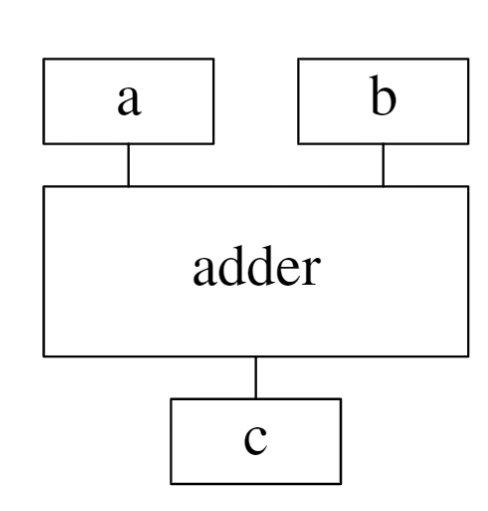
\includegraphics[width= 100px]{images/Screenshot 2024-01-08 151414.png}
\end{center}
This hardware can add two numbers, that is, conduct the operation $c=a+b$. It could also perform $f=d+e$ or $i=g-h=g+(-h)$ as it is not restricted to the sole values of $a$ and $b$ as inputs. This process fits into the logic design and switching algebra portions of chip manufacturing.\\
The creation of systems like these is based on the fact that voltage and current are time-varying and can assume any value in a continuous range of real numbers, but are mapped to only two values.

\subsection{Digital Logic Signals}
A digital signal is modeled assuming that at anytime, it can have only one of
two discrete values, which represent:\\
\begin{table}
    \centering
    \begin{tabular}{c|c}
        0     & 1    \\
        LOW   & HIGH \\
        FALSE & TRUE \\
    \end{tabular}
\end{table}
This is called positive logic.
It maps the infinite values of voltage and current to these two values.
An example of this is CMOS 2-Volt logic:\\
\begin{table}
    \centering
    \begin{tabular}{c|c}
        0      & 1        \\
        \hline
        0-0.5V & 1.5-2.0V \\
    \end{tabular}
\end{table}
These completely separated ranges of values allow for 0 and 1 to be completely separate, with noise and other possible errors being ignored. In this way, all physical values can be partitioned into the two values, though, for intents and purposes of digital system design, voltage is the most relevant.\\
Additionally, circuits known as buffer circuits can be used to restore logic values. That is, if a voltage is not sufficiently close to the values of 0 or 2 (in the case of the CMOS), they can push these values far closer to the desired values, reducing the possibility of error.\\
Digital circuits have replaced analog circuits becuse they are far easier to design. They can be made using Hardware Description Languages (HDLs), softwares that are similar to programming languages.\\
A logic value is called a binary digit, or bit. A set of $n$ bits, represent $2^n$ values. For example:
\begin{table}
    \centering
    \begin{tabular}{c}
        $b_0$ \\
        \hline
        0     \\
        1     \\
    \end{tabular}
    \quad
    \begin{tabular}{c c}
        $b_0$ & $b_1$ \\
        \hline
        0     & 0     \\
        1     & 0     \\
        0     & 1     \\
        1     & 1
    \end{tabular}
\end{table}
\subsection{Logic Circuits}
At the highest level, a logic circuit is a \textit{black box} with $n$ inputs
and $m$ outputs. Only zeros and ones are required to represent inputs and
outputs. \\ Combinational circuits are circuits that have outputs that solely
depend on the inputs. It can be represented by a truth table.\\ An adder can be
represented by a truth table in this manner.
\begin{center}
    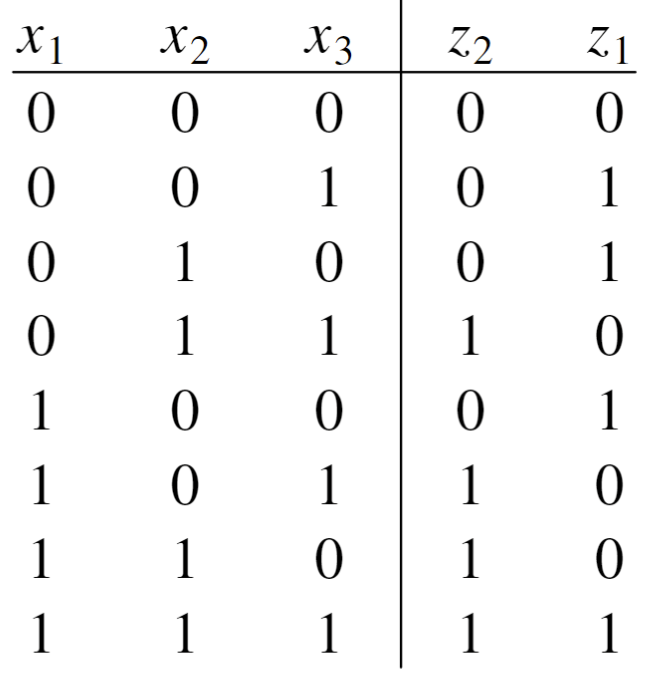
\includegraphics[width= 100px]{images/Screenshot 2024-01-10 144557.png}
\end{center}
On the other hand, a sequential circuit has memory. That is, the output is dependent on both the inputs and the current state of the circuit itself. This is representable through a state table.\\
\begin{center}
    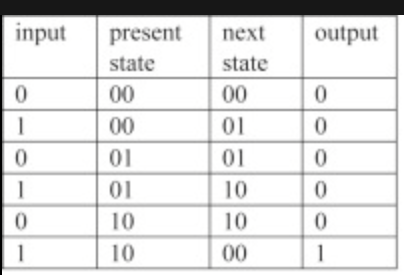
\includegraphics[width= 150px]{images/state table.png}
\end{center}
\subsection{Gates}
Basic digital devices are called gates. These implement basic logic functions.
These are AND, OR, NOT. However, AND, NOT and OR, NOT are sufficient to make
any combination, as the third gate can be formed as a combination of the other
two.\\ Each of the gates is represented symbolically like the following, and
have their truth tables shown below:\\
\begin{table}
    \centering
    \begin{tabular}{c|c|c}
        AND                                                & OR                                                & NOT                                                \\
        \hline
        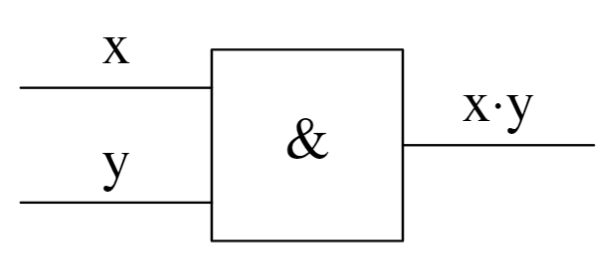
\includegraphics[width= 80px]{images/AND_GATE.png} & 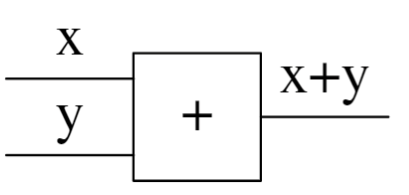
\includegraphics[width= 80px]{images/OR_GATE.png} & 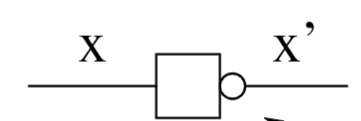
\includegraphics[width= 80px]{images/INVERTER.png} \\
        \hline
        \begin{tabular}{c c|c}
            x & y & {$x\land y$} \\
            \hline
            0 & 0 & 0            \\
            0 & 1 & 0            \\
            1 & 0 & 0            \\
            1 & 1 & 1
        \end{tabular}                            &
        \begin{tabular}{c c|c}
            x & y & {$x\lor y$} \\
            \hline
            0 & 0 & 0           \\
            0 & 1 & 1           \\
            1 & 0 & 1           \\
            1 & 1 & 1
        \end{tabular}                             &
        \begin{tabular}{c|c}
            x & {$\lnot x$} \\
            \hline
            0 & 1           \\
            1 & 0           \\
        \end{tabular}
    \end{tabular}
\end{table}
This can be done for more inputs, by combining multiple gates.\\ There are two more often used gates that can be created through a combination of these two.\\
\begin{table}
    \centering
    \begin{tabular}{c|c}
        NAND                                                & NOR                                                \\
        \hline
        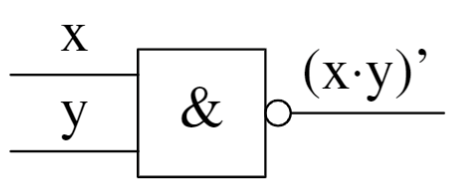
\includegraphics[width= 80px]{images/NAND_GATE.png} & 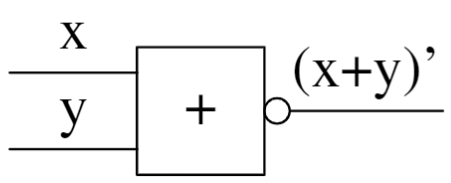
\includegraphics[width= 80px]{images/NOR_GATE.png} \\
        \hline
        \begin{tabular}{c c|c}
            x & y & {$\lnot(x\land y)$} \\
            \hline
            0 & 0 & 1                   \\
            0 & 1 & 1                   \\
            1 & 0 & 1                   \\
            1 & 1 & 0
        \end{tabular}                &
        \begin{tabular}{c c|c}
            x & y & {$\lnot(x\lor y)$} \\
            \hline
            0 & 0 & 1                  \\
            0 & 1 & 0                  \\
            1 & 0 & 0                  \\
            1 & 1 & 0
        \end{tabular}
    \end{tabular}
\end{table}
It is a good exercise to see how two of the basic gates (AND, NOT or OR, NOT) can be used to create the rest, as it is possible to connect gates to form complex circuits and thus, complex functions.\\
\textit{Note: By convention, signal flows from left to right. Thus, output comes out the right and input goes in at left.}
\subsection{Timing}
When the values of an input changes, it takes time for the outputs to change as
well, which is known as \textit{propagation delay}, which can be represented in
a timing diagram. However, for most cases, it is possible ot ignore these, as
the behavior is well defined regardless of delay.\\ The following is a timing
diagram:\\
\begin{center}
    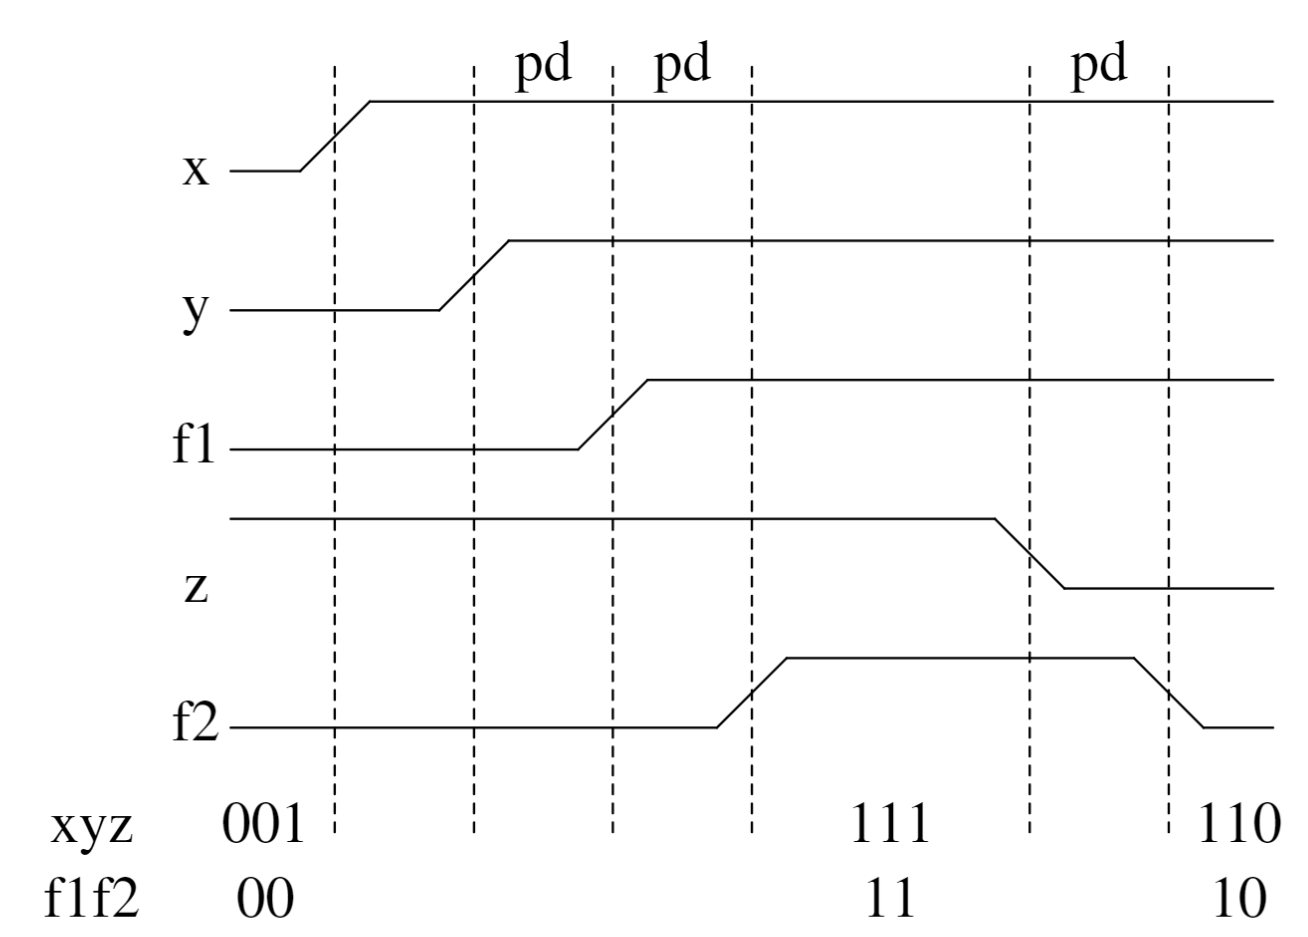
\includegraphics[width= 200px]{images/timing_table.png}
\end{center}
Propagation delay, represented by pd in the timing diagram, is irrelevant if there are no changes, regardless of the fact that there is a new set of inputs. The values at the bottom of the diagram are the values that each of the elements hold after all the necessary transitions have happened for that set of inputs.\\
Transition time is the time it takes for a signal to change from 0 to 1, and is represented by "rt".
\subsection{Software Aspects of Digital Design}
Software is not technically essential to digital system design. People used to
draw symbold by hand, and could make technically equivalent systems. However,
the availability, utility, and ease of use of HDLs has made the use of software
prevalent in the current technological landscape.\\ Electronic Design
Automation tools are useful in improving designer productivity. The following
are examples of these:
\begin{itemize}
    \item Schematic entry: Allows for fully detailed digital diagrams to be created
          digitally.
    \item HDLs: Can be used to design anythong from individual function modules to
          multichip digital systems. This course will involve extensive use of VHDL.
    \item HDL text editors, compilers, synthesizers: text editor to define, compiler to
          debug syntax, synthesizer to create corresponding circuit or chip.
    \item Simulator: It is virtually impossible to debug a synthesized chip, so
          simulators are used before synthesis. They allow for verification of
          functionality prior to the actual tedious process of synthesis. Among
          simulators, there are also PCB simulators, and FPGAs, which are like
          programmable chips. They are very important.
    \item Test benches: Designs are simulated and tested using these. They run a series
          of checks to ensure that nothing stopped working due to changes.
    \item Timing analyzers and verifiers: Correct timing of inputs and reactiosn are
          paramount in digital systems. This facet of simulation allows for the
          automation of timing functionality verification.
    \item Word Processors: Allow for pretty documentation to be created.
\end{itemize}
Software is important, but the understanding of what it actually does is even more so.
\subsection{Integrated Circuits}
A collection of gates on a single silicon chip is called an integrated circuit
or IC.\\ An IC originates from a wafer, which is segmented into many identical
ICs. The wafer is divided into rectangles, called \textit{dies} which in turn
have \textit{pads} which allow for wire connections. Microscopic probes are
used to debug the wafers, and defects are discarded, and the succeses, cut
out.\\ For this class, an IC, is a packaged die.\\ ICs were divided by size,
small SSIs with 1 to 20 gates, medium MSIs with 20 to 200, large LSIs with upto
1000, and vely large VLSIs fro everything above that. The largest VLSIs now
have over 10 billion transistors.\\ An IC process is the steps taken to create
an IC, and are categorized by the transistor density within the chip.
\subsection{Logic Families}
There are many different ways of implementing logic circuits. Connectable logic
circuits are of the same logic family. So, the technology controlling them is
different. Chips need to be from the same family to be connected to each other.
If they are from different families, they cannot be connected to each other.\\
For example TTL (Transistor-Transistor Logic) is a logic family based on
bipolar junction transistors.\\ CMOS (Complementary Metal-Oxide Semiconductor)
is based on MOSFETs (MOS Field-Effect Transistors). These are more commonly
used, and the ones we will be analyzing in this class.\\
\subsection{CMOS Logic Circuits}
A MOS transistor is modellable as a voltage controlled resistor. This means
that the input voltage controls the resistance of the MOSFET, allowing it to
act as a kind of switch. This is because it has only two effective states: very
high resistance and very low resistance.\\ This is an n-channel (NMOS)
transistor:
\begin{center}
    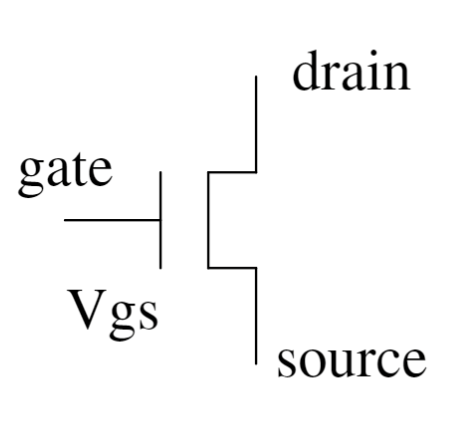
\includegraphics[width= 100px]{images/nmos.png}
\end{center}
When $V_{gs} = 0$, the resistance is very high.\\
When $V_{gs}$ is increased, the resistance is very low.\\
On the other hand, this is the PMOS transistor:\\
\begin{center}
    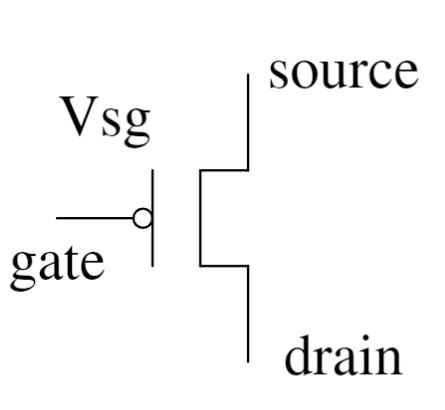
\includegraphics[width= 100px]{images/pmos.png}
\end{center}
When $V_{sg} = 0$, the resistance is very high.\\
When $V_{sg}$ is increased, the resistance is very low.\\
NMOS and PMOS together allow us to form CMOS logic.
For example, this is a CMOS inverter, in which the output will be the opposite of the input.\\
\begin{center}
    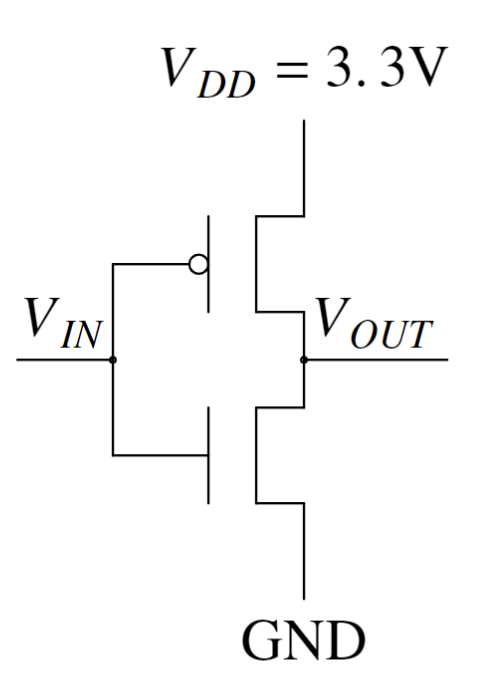
\includegraphics[width= 100px]{images/cmosinverter.png}
\end{center}
If $V_{in} = 3.3V$, or high, the PMOS transistor be off, and the NMOS would be on. This would mean that the output and ground are shorted, causing the output to be low.\\
If $V_{in} = 0V$, or low, the PMOS transistor be on, and the NMOS would be off. This would mean that the output and $V_{DD}$ are shorted, causing the output to be high.\\
This allows this to be act as an inverter.\\
Now we will observe the CMOS arrangement of a NAND gate.
\begin{center}
    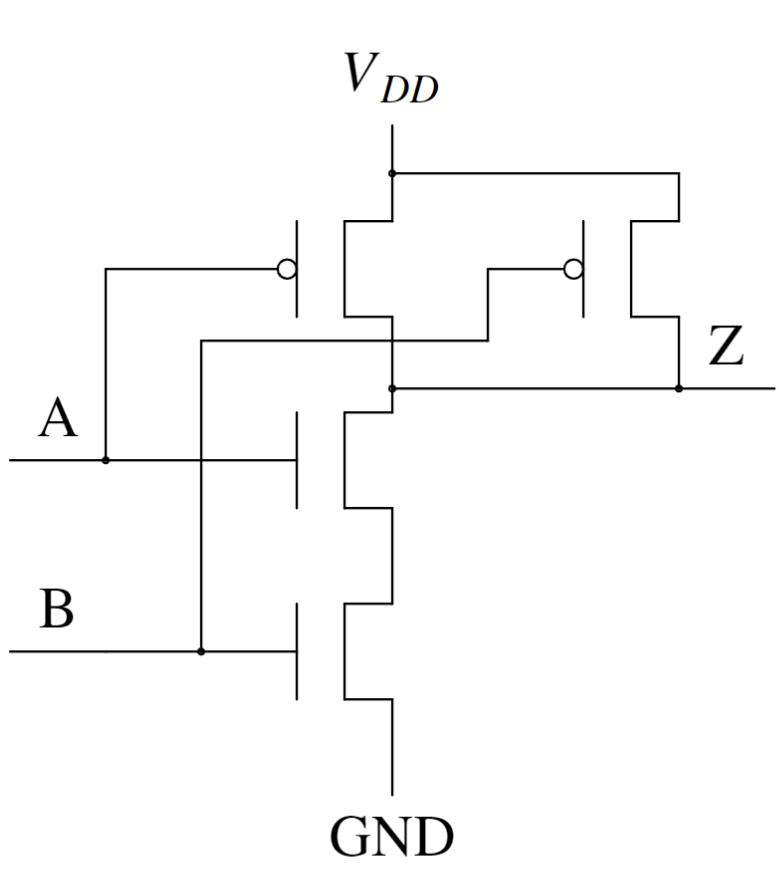
\includegraphics[width= 150px]{images/cmosnand.png}
\end{center}
If A and B are both HIGH, both PMOS are HIGH, and thus $V_{DD}$ is shorted to Z.\\
If they are both LOW, the exact opposite happens, with Z shorting to ground.\\
If A or B are HIGH, than one of the PMOS will be high, and one of the NMOS will be LOW, causing the output to be HIGH.\\
The NOR gate can be constructed easily from the same thought process, but NMOS in parallel, and PMOS in series.\\
These can be expanded to more inputs by adding more transistors.\\
\subsection{Preview of future topics}
%Fan-in is the number of inputs that a gate has. As it increases, the resistances of the transistors increase, and thus, the delay.
The following is a multiplexer:
\begin{center}
    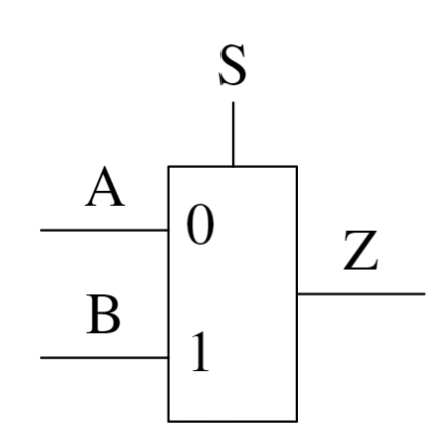
\includegraphics[width= 100px]{images/multiplexer.png}
\end{center}
It outputs A when S is 0, and B when S is 1. It allows us to select between different functions, such as adding and subtracting.\\
Truth tables are another form of representation of a digital system. We will later learn how to analyze and derive equations from truth tables, as well as the gate implementation.\\
\textit{Note: CMOS logic doesn't have AND, OR gates, so the actual implementation of these two is NAND, NOR gates with an inverter.}\\
Gates require 4 transistors, and inverters need two transistors.
Verilog Structural model:
\begin{lstlisting}
    module Ch1mux_s(A,B,S,Z);
        input A,B,S;
        output Z;
        wire SN,ASN,SB;
        not U1(SN,S);
        and U2(ASN,A,SN);
        and U3(SB,B,S);
        or U4(Z,ASN,SB);
    endmodule
\end{lstlisting}
Which is equivalent to:
\begin{center}
    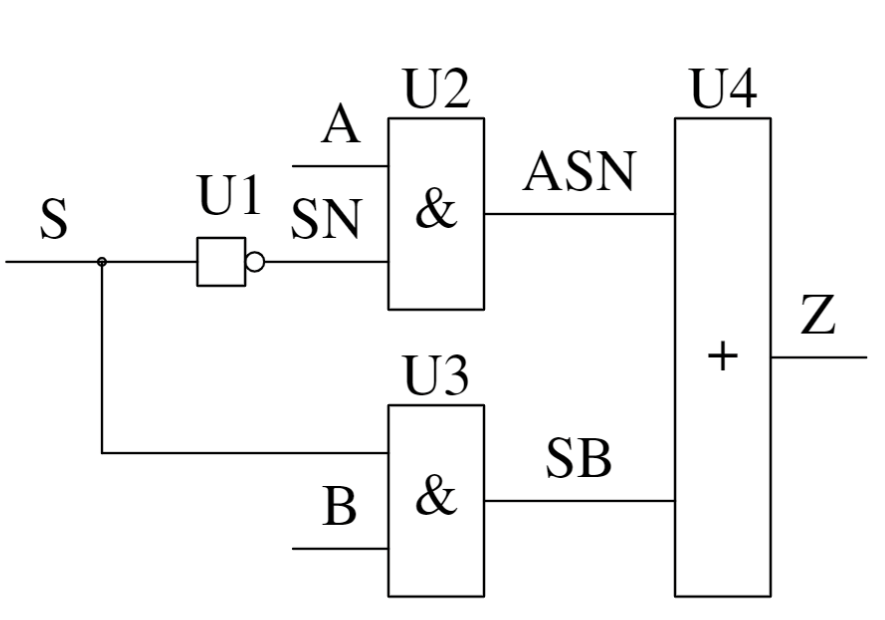
\includegraphics[width= 150px]{images/verilog_implementation.png}
\end{center}
\textit{Note: the order of these statements is irrelevant, they will result in the same digital system.}
Verilog Behavioral Model:
\begin{lstlisting}
    module Ch1mux_b(A,B,S,Z);
        input A,B,S; \\input declaration
        output reg Z; \\output declaration
        always @(A,B,S) \\if input changes, recompute
        if (S==1) Z=B; 
        else Z=A; \\this is saying what the multiplexer above did
    endmodule
\end{lstlisting}
\section{Number Systems and Codes}
A digital circuit processes binary digits in the form of bits.\\ It is
impoortant to see how these relate to real life values.\\ Numbers in the
decimal system:
\begin{equation*}
    abcd = 1000a+100b+10c+d = 10^3a+10^2b+10^1c+10^0d
\end{equation*}
The base, or radix is 10.
For a general radix $r$, it would be:
\begin{equation*}
    abcd = r^3a+r^2b+r^1c+r^0d
\end{equation*}
For this course, we care about binary, or radix 2.\\
Occasionally, base 8 (octal) and base 16 (hexadecimal) are also relevant.
\begin{table}
    \centering
    \begin{tabular}{c|c|c}
        base 2 & base 8 & base 16 \\
        \hline
        0      & 0      & 0       \\
        1      & 1      & 1       \\
        10     & 2      & 2       \\
        11     & 3      & 3       \\
        100    & 4      & 4       \\
        101    & 5      & 5       \\
        110    & 6      & 6       \\
        111    & 7      & 7       \\
        1000   & 10     & 8       \\
        1001   & 11     & 9       \\
        1010   & 12     & A       \\
        1011   & 13     & B       \\
        1100   & 14     & C       \\
        1101   & 15     & D       \\
        1110   & 16     & E       \\
        1111   & 17     & F       \\
    \end{tabular}
\end{table}
To convert from octal to binary, replace every octal with three bits starting from the least significant bit.  For hexadecimal, replace each digit with 4 bits.\\
The least significant bit(LSB) is the last bit, and the first is the most significant bit (MSB).\\
To convert from decimal to binary by dividing the number by 2, and assigning the remainder to the least siginificant unassigned bit. Do this continuously to the quotient until done.\\
\subsection{Adding and Subtracting}
To add and subtract in binary:\\
\begin{table}
    \centering
    \begin{tabular}{c c c c c c}
          & 1 & 0 & 1 & 1 & + \\
          & 1 & 0 & 1 & 0 &   \\
        \hline
        1 & 0 & 1 & 0 & 1
    \end{tabular}
    \quad\quad
    \begin{tabular}{c c c c c c}
        1 & 1 & 0 & 1 & 1 & - \\
          & 1 & 0 & 1 & 0 &   \\
        \hline
        1 & 0 & 0 & 0 & 1 &
    \end{tabular}
\end{table}
To add signs to numbers, it has been standardized that the first bit defines the sign. If the leftmost bit is 0, the number is posititve. and if it is 1, the number is negative. \\This allows an n-bit signed integer to be from the range $-2^{n-1}+1 \text{ to } 2^{n-1}-1.$\\
To actually add and subtract numbers, we first check if the sign is the same, if it is, we add directly, and append the sign bit. If they have opposing signs, we find the larger number, subtract the smaller, and use the sign of the larger.\\
\subsection{Using the complement to conduct operations}
In the complement number system, we can add or subtract directly, the
operations can be done directly. The complementation process is more
complicated than sign checking, but it simplifies addition.\\ The 2-complement
system is the difference between $2^n$ and the n-bit integer. To compute $-B$,
we first need to calculate $2^n-B$, which we can compute as $(2^n-1)-B+1$,
which is essentially inverting each bit, and adding 1 to the result. (Carries
outside the bit length are ignored.)\\ The most significant bit of the
complement acts as a sign bit. This can be seen in the following table:
\begin{table}
    \centering
    \begin{tabular}{c c|c c}
        number & binary & negative & binary \\
        \hline
        0      & 0000   & -0       & 0000   \\
        1      & 0001   & -1       & 1111   \\
        2      & 0010   & -2       & 1110   \\
        3      & 0011   & -3       & 1101   \\
        4      & 0100   & -4       & 1100   \\
        5      & 0101   & -5       & 1011   \\
        6      & 0110   & -6       & 1010   \\
        7      & 0111   & -7       & 1001   \\
        -      & -      & -8       & 1000   \\

    \end{tabular}
\end{table}
The magnitude of a number can be computed as for an unsigned number, except that the weight of the MSB is $-2^{n-1}$ instead of $2^{n-1}$. So, to subtract $2^n$, replace the weight of the MSB with $-2^{n-1}$.\\
To add a bit to a complement number, we can simply duplicate the MSB at the beginning of the MSB.
As proof of this actually working, we can calculate the complement of both the complement and the modified complement as uncomplemented numbers, and we can observe that they will be the same.\\
That is, the complement of 11001 and 111001 is the same number, the same happens for 011 and 0011.\\
We can also reverse this process if the digits corresponding to the removed bits of the given complement are all the same.\\
Now we will analyze how the complement can be used to add and subtract.\\
\begin{center}
    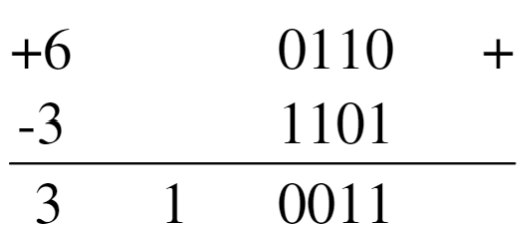
\includegraphics[width = 100px]{images/add_complement.png}
\end{center}
This process may not work if overflow occurs. That is, if the number of necessary bits to represent the result of an operation are more than the available bits. This can only occur if the numbers being operated on have the same sign.\\
To subtract two numbers, we instead use the following property: $X-Y = X+(-Y) = X+Y'+1$ where $Y'$ is the complement of $Y$.
\begin{center}
    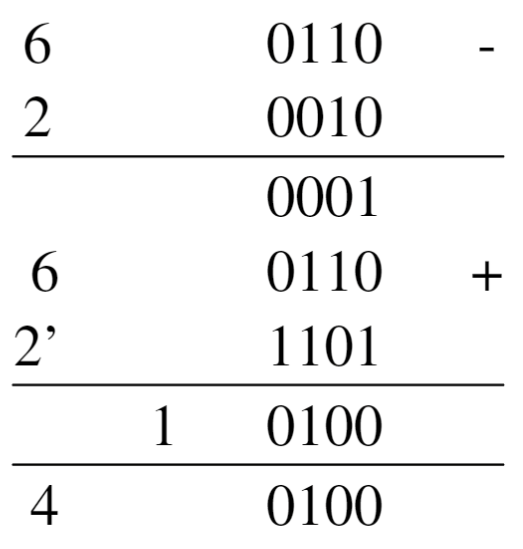
\includegraphics[width = 100px]{images/complement_subtraction.png}
\end{center}
\subsection{Binary Codes for Decimal Numbers}
A set of \textit{n}-bit strings in which differnt bit strings represent
diffferent elements of a set is called a code. A combination on these is a code
word.\\ 0 through 9 requires at least 4 bits, but there are many methods of
doing so.\\
\begin{center}
    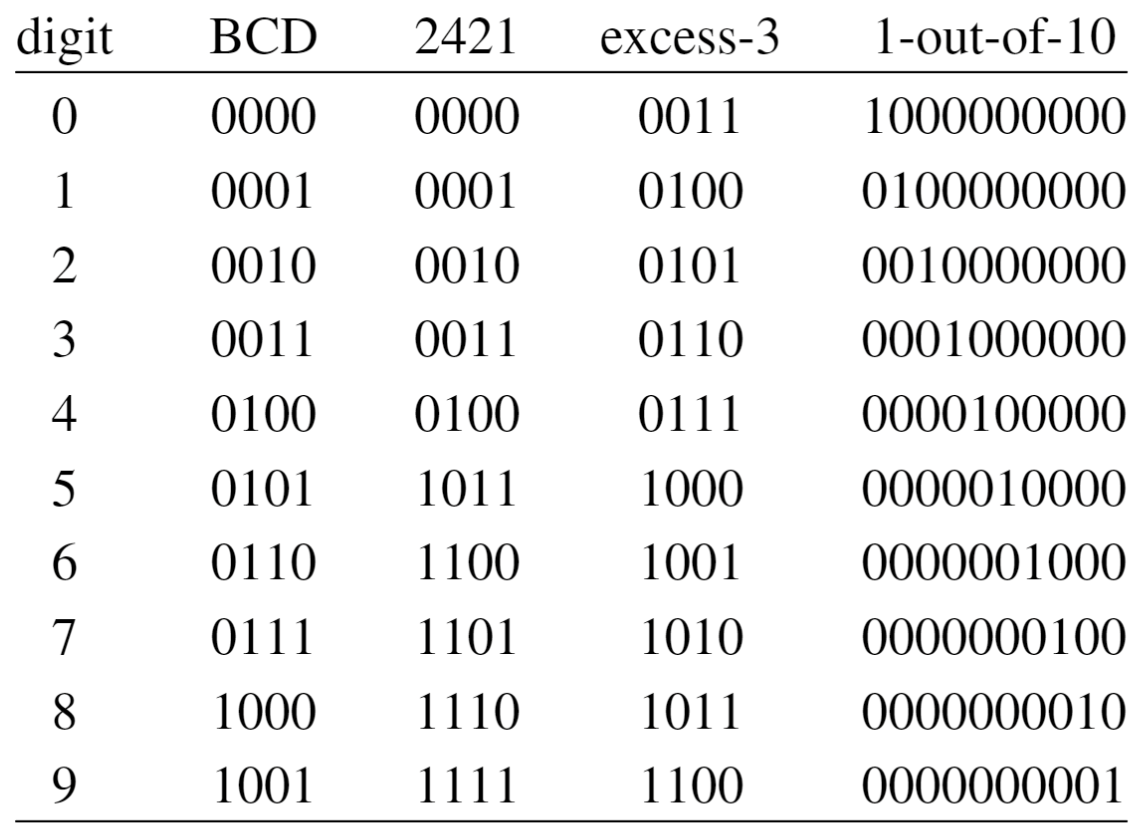
\includegraphics[width = \textwidth]{images/decimal_codes.png}
\end{center}
Another very important representation is the gray code.\\
By partitioning a disk into eight regions, with n bits with sensors in each, any number between 0 and $2^n -1$ can be represented.\\
\begin{center}
    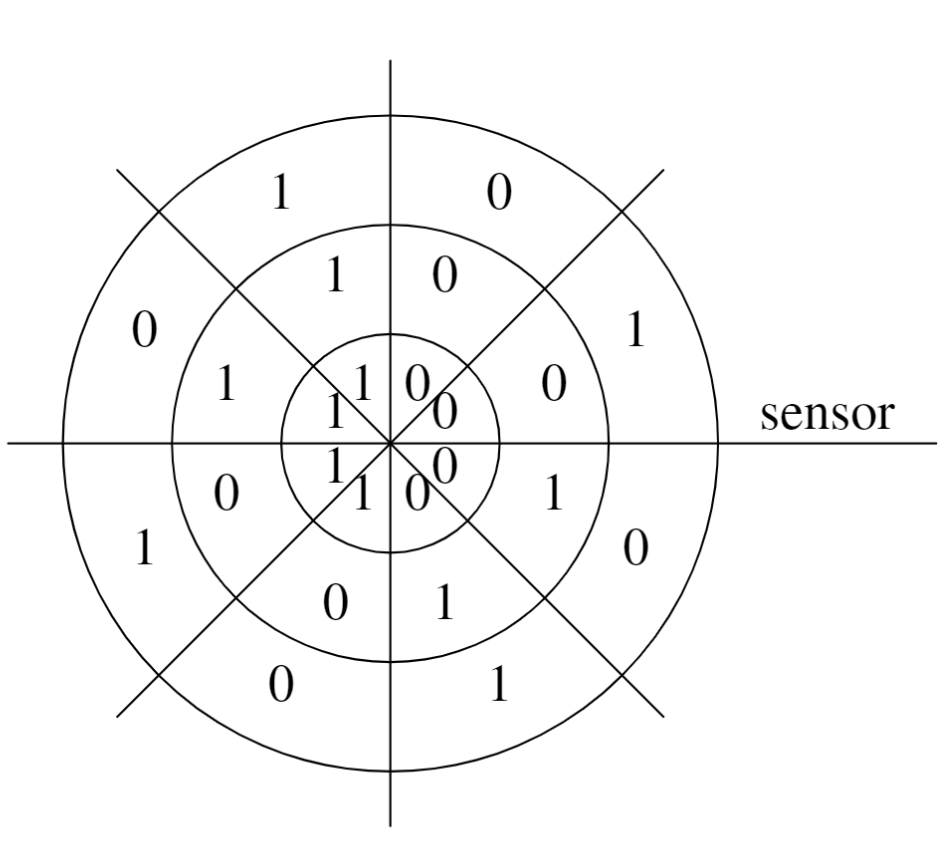
\includegraphics[width = 200px]{images/gray_code.png}
\end{center}
\textit{Note: if the disk stops between two sections, there is a possibility of error. Using standard binary representation will cause the error to be very large, as it can stop between 000 and 111, which would imply that any of the bits can have error, and thus any of the numbers between 0 and 7 can be represented.}
This is where the gray code comes in:\\
\begin{table}
    \centering
    \begin{tabular}{c|c}
        number & gray code \\
        \hline
        0      & 000       \\
        1      & 001       \\
        2      & 011       \\
        3      & 010       \\
        4      & 110       \\
        5      & 111       \\
        6      & 101       \\
        7      & 100       \\
    \end{tabular}
\end{table}
This encoding allows there to be only one bit of change between any two consecutive digits, allowing us to reduce the margin of error.\\
Codes can also be used to represent text, as the ASCII does, which uses a 7-bit code word.\\
The selection of code and code words is very important, as it can drastically change the complexity of the designed circuit:
\begin{center}
    \centering
    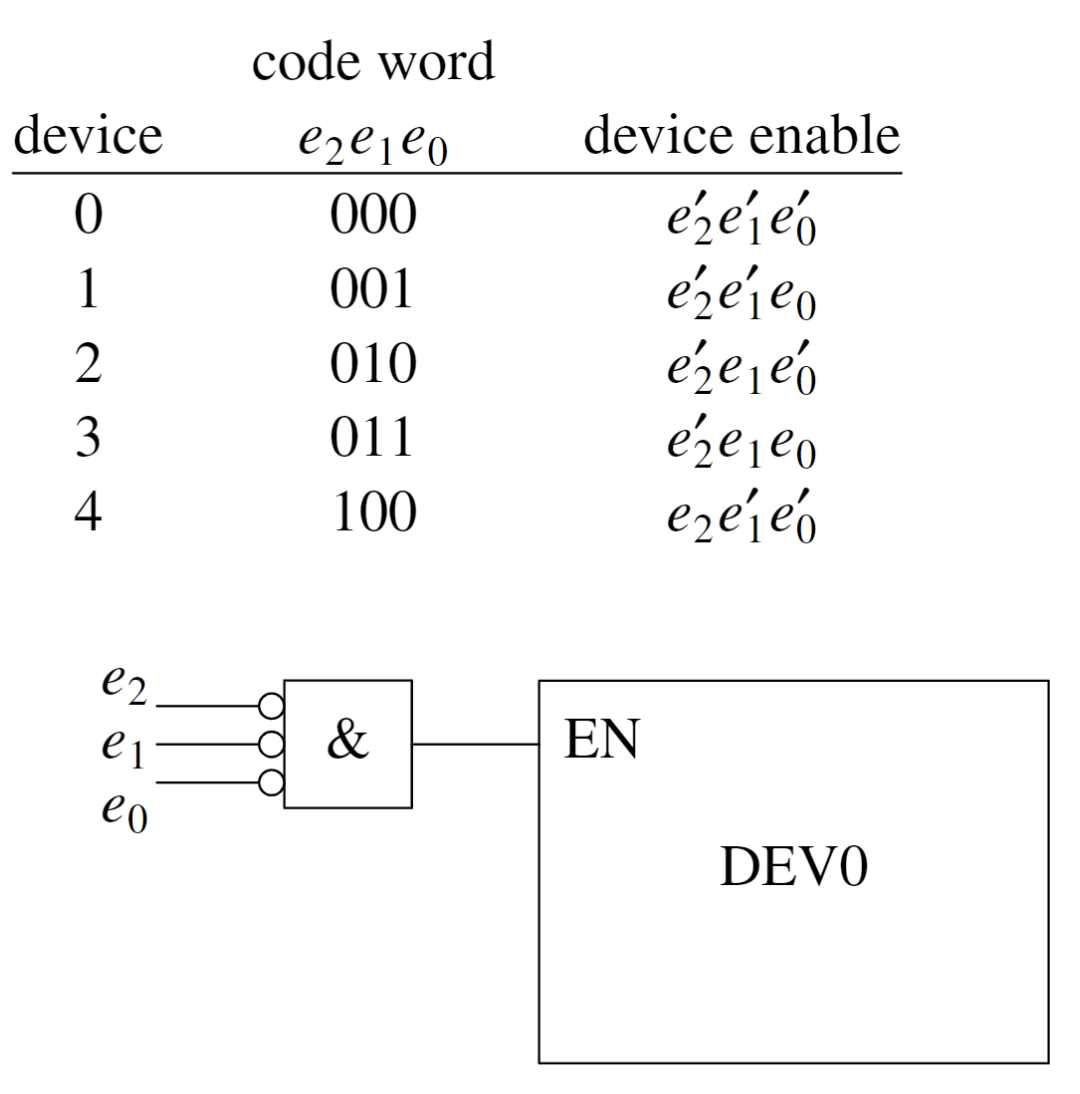
\includegraphics[width = 100px]{images/code_ex1.png} \quad
    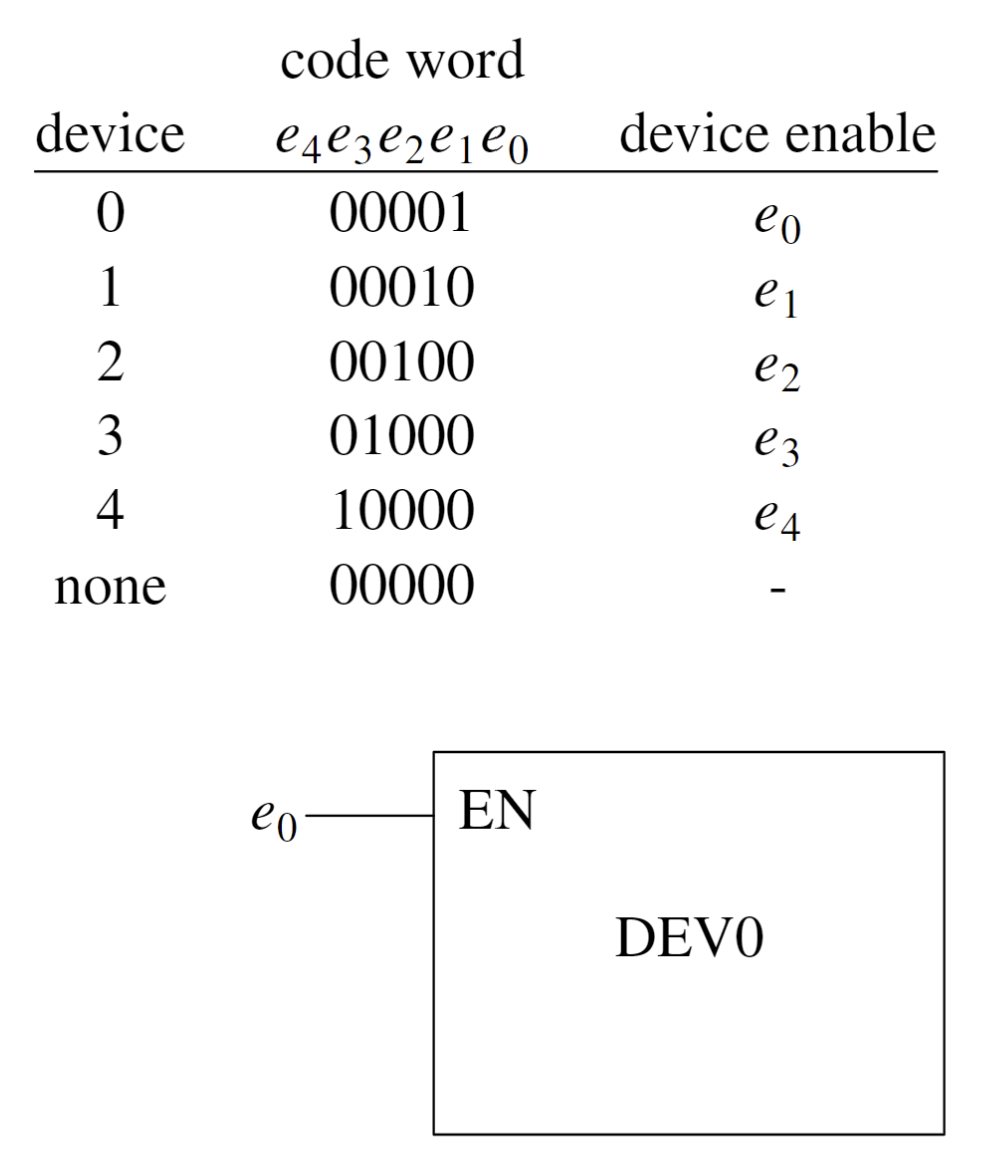
\includegraphics[width = 100px]{images/code_ex2.png}
\end{center}
\section{Switching Algebra and Combinational Logic}
A combinational circuit depends only on the inputs. We will begin by
considering single ouptut combinational circuits.\\ Switching algebra is a
mathematical tool used for circuit design. It is a subset of boolean algebra. A
variable is used to represent a signal.\\
\subsection{Axioms}
\begin{itemize}
    \item (A1) $X=0$ if $X \neq 1$
    \item (A1D) $X=1$ if $X \neq 0$
\end{itemize}
There is a principle of duality in this axiom, as do most properties of switching algebra.\\
\begin{itemize}
    \item (A2) $X=0 \implies X' = 1$
    \item (A2D) $X=1 \implies X'=0$
    \item (A3) $0 \land 0 = 0$
    \item (A4) $1 \land 1 = 1$
    \item (A5) $0\land 1 = 1\land 0 = 0$
    \item (A6) $ 1 \lor 1=1$
    \item (A7) $0\lor 0 = 0$
    \item (A8) $1\lor 0 = 0\lor 1 = 1$
\end{itemize}
AND has a higher precedence than OR in logical expressions"
\begin{equation*}
    W\land Y \lor Y\land Z = (W\land X) \lor (Y\land Z)
\end{equation*}
\subsection{Theorems}
There are 5 theorems that can be easily be proven through this:
\begin{enumerate}
    \item $X\lor 0=X$
    \item $X \lor 1 = 1$
    \item $X \lor X = X$
    \item $(X')'=X$
    \item $X\lor X' = 1$
\end{enumerate}
Which have the following dualities:
\begin{enumerate}
    \item $X\land 1 =X$
    \item $X\land 0 = 0$
    \item $X \land X = X$
    \item No duality
    \item $X\land X' = 0$
\end{enumerate}
There are also two variable theorems:
\begin{itemize}
    \item Commutativity:
          \begin{enumerate}
              \item $X\lor Y=Y\lor X$
              \item $X\land Y = Y\land X$
          \end{enumerate}
    \item Associativity: \begin{enumerate}
              \item $(X\lor Y)\lor Z=X\lor (Y\lor Z)$
              \item $(X\land Y)\land Z=X\land (Y\land Z)$
          \end{enumerate}
          This allows for the representation of three or more input gates with ease.
    \item Distributivity:
          \begin{enumerate}
              \item $X\land Y \lor X\land Z = X\land(Y \lor Z)$
              \item $(X\lor Y)\land (X\lor Z) = X\lor Y\land Z$
          \end{enumerate}
    \item Covering:
          \begin{enumerate}
              \item $X\lor X\land Y = X$
              \item $X\land(X\lor Y) = X$
          \end{enumerate}
    \item Combining:
          \begin{enumerate}
              \item $X\land Y \lor X\land Y' = X$
              \item $(X\lor Y)\land (X\lor Y')=X$
          \end{enumerate}
    \item Consensus:
          \begin{enumerate}
              \item $X \land Y \lor X' \land Z \lor Y \land Z = X \land Y \lor X' \land Z$
              \item $(X \lor Y ) \land (X' \lor Z ) \land (Y \lor Z ) = (X \lor Y ) \land (X' \lor Z)$
          \end{enumerate}
\end{itemize}
All these theorems can be proven using perfect induction, that is, through building the complete truth table for the inputs, and showing that the output is always true.\\
Some of these can also be proven using the axioms and priorly proven theorems.
\textit{Note: The proof of one theorem, can be applied to the dual, but using the duals of the theorems used in the proof of the first.}
\begin{itemize}
    \item Variable Theorems:
          \begin{enumerate}
              \item $X\lor X\lor X \ldots \lor X = X$
              \item $X\land X\land X \ldots \land X = X$
          \end{enumerate}
    \item De Morgan's Theorems:
          \begin{enumerate}
              \item $(X_1\land X_2\land X_3 \ldots \land X_n)'=X_1'\lor X_2'\lor X_3' \ldots \lor X_n'$
              \item $(X_1\lor X_2\lor X_3 \ldots \lor X_n)'=X_1'\land X_2'\land X_3' \ldots \land X_n'$
          \end{enumerate}
\end{itemize}
Using De Morgan's Theorems allows us to change combinations of NANDs and NORs into more efficient NAND only or NOR only gate functions.\\
\textbf{De Morgan's Theorem Generalization:}
\begin{equation*}
    [F(X_1, X_2, . . . , X_n, \lor, \land)]'= [F(X_1', X_2', . . . , X_n', \land, \lor)]
\end{equation*}
\begin{itemize}
    \item Shannon's Expansion theorems:
          \begin{enumerate}
              \item $F(X_1, X_2, . . . , X_n) =X_1 \land F(1, X_2, . . . , X_n) \lor X_1' \land F(0, X_2, . . . , X_n)$
              \item $F(X_1, X_2, . . . , X_n) =X_1 \lor F(1, X_2, . . . , X_n) \land X_1' \lor F(0, X_2, . . . , X_n)$
          \end{enumerate}
\end{itemize}
These can be proven through finite induction.
\subsection{Connecting Switching Algebra and Combinational Logic}
We will start by defining some things:\\
\begin{itemize}
    \item A \textit{literal} is a variable that can be complemented or uncomplemented,
          for example $X,X',Y,Y'$
    \item A \textit{product term} is a literal or a product (AND) of two or more
          literals, for example $X,X',X\land Y'\land Z$
    \item A \textit{sum-of-products} is a sum (OR) of multiple products.
    \item A \textit{sum term} is a single literal or the sum (OR) of multiple literals.
    \item A \textit{product-of-sums} is a product of multiple sum terms.
    \item A \textit{normal term} is a product or sum in which no variable appears more
          than once.
    \item An \textit{n-variable minterm} is a normal product term with n literals. There
          are $2^n$ such terms. That is, each variable appears exactly once in the term,
          in either complemented or uncomplemented form. It is 1 in only one row of the
          truth table.
    \item An \textit{n-variable maxterm} is a normal sum term with n literals. Once
          again, there are $2^n$ such terms. It is 0 in only one row of the truth table.
    \item A \textit{canonical sum} of a function is the sum of the minterms corresponding
          to the rows where the truth-table of the function is 1.
          \begin{center}
              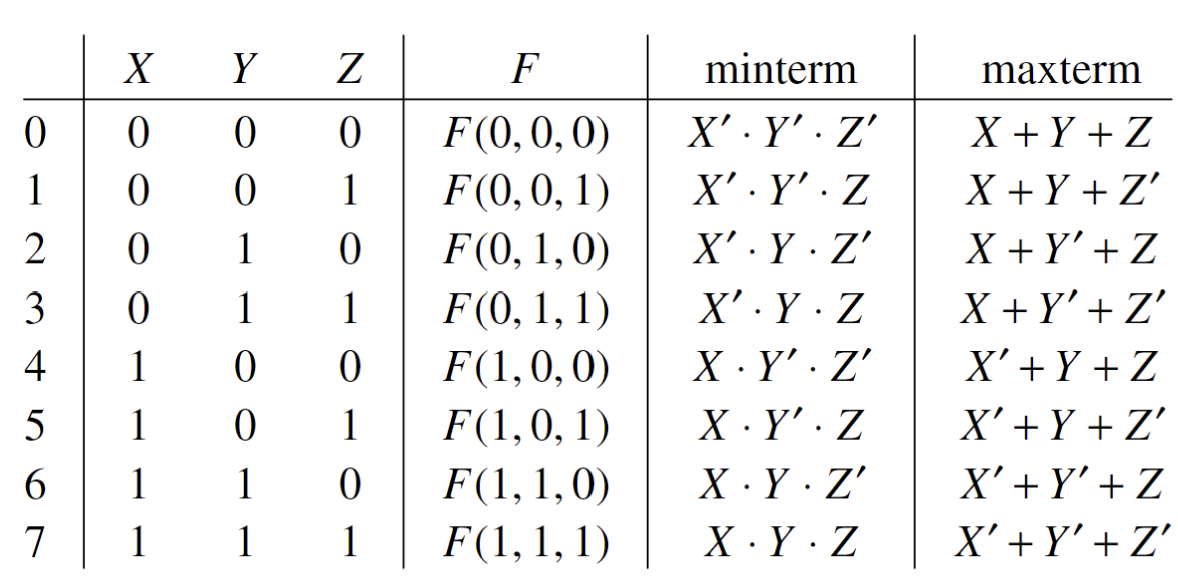
\includegraphics[width = 150px]{images/minterm_maxterm_func.png}
          \end{center}
          This has another notation, in which each row that is true is added to the sum:
          \begin{equation*}
              F = (1,0,0,1,1,1,0,1)=\sum_{X,Y,Z}(0,3,4,5,7)
          \end{equation*}
    \item A \textit{canonical product} of a function is the product of the maxterms
          corresponding to the truth table rows where the function is 0.
          \begin{center}
              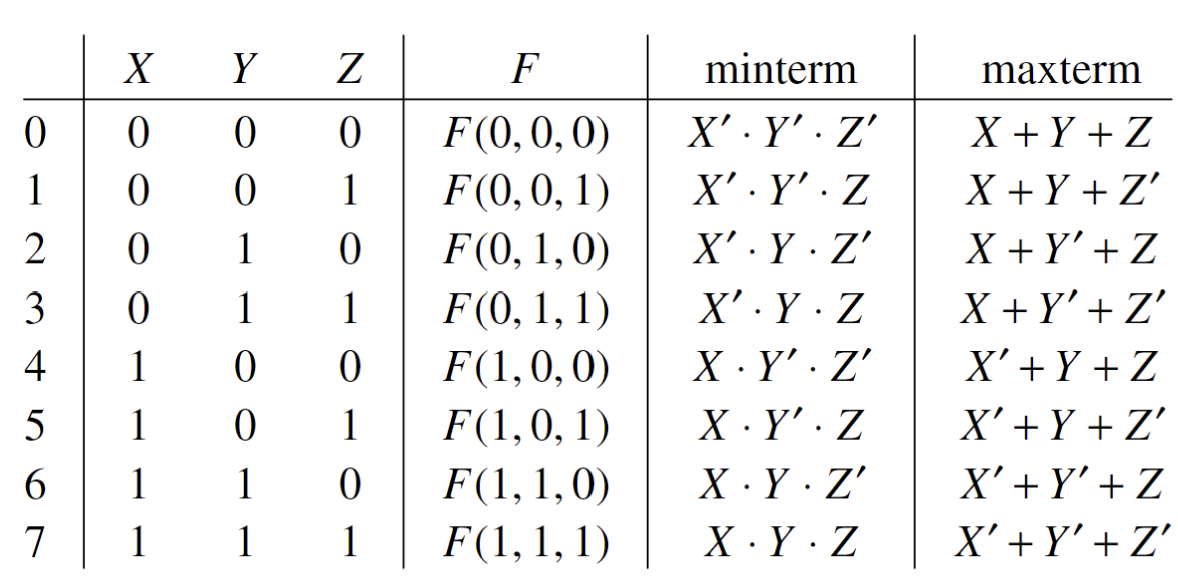
\includegraphics[width = 150px]{images/minterm_maxterm_func.png}
          \end{center}
          This also has another notation:
          \begin{equation*}
              F = (1,0,0,1,1,1,0,1)=\prod_{X,Y,Z}(1,2,6)
          \end{equation*}
          \begin{center}
              \textit{Note: the union of the terms of the canonical product and the canonical sum, is the full truth table, or the numbers from $0\rightarrow 2^n-1$}
          \end{center}
\end{itemize}
A function can be written in Verilog by doing the following:
\begin{lstlisting}
    case{(X,Y,Z)}
        0,3,4,5,7:F=1;
        default:F=0;
    endcase
\end{lstlisting}
Or it can be written like this:
\begin{lstlisting}
    case{(X,Y,Z)}
        1,2,6:F=;
        default:F=1;
    endcase
\end{lstlisting}
Now that we have all the necessary definitions, we will go back to Shannon's
Expansion Theorem.
\begin{equation*}
    F(X_1, X_2, . . . , X_n) =X_1 \land F(1, X_2, . . . , X_n) \lor X_1' \land F(0, X_2, . . . , X_n)
\end{equation*}
This theorem allows us to extract a variable from a function and divide it into two halves, in which the term is true or false, while the remains have a smaller minterm, maxterm truth table.\\
\subsection{Combinational Circuit Analysis}
Circuit analysis is defined as locating the logic function that defines it. It
is the transition from a logic diagram to a truth table or an algebraic
expression.\\ Once this function is available, it can be used to determine the
behavior, or manipulate the circuit for more efficiency, or for different
elements. For example, it may be necessary to modify a circuit to transition
from PLA to FPGA.\\ To do so, all functions to be compared are reduced to the
canonical form, as it is unique.\\ One method of running analysis on a logic
circuit, we can analyze its output for each of the $2^n$ inputs it can get, and
find the output. However, this is no longer viable for large values of $n$.\\
The other method would be to find the output of each gate, starting from the
left towards the right of the circuit, each output is joined to find the end
function of the circuit. The function can then be minimized and made more
efficient.\\ DeMorgan's theorem can be used to simplify circuits, for example,
it can allow us to replace a NAND gate with an OR gate with inverted inputs, or
NOR gates with AND with inverted inputs. This is usually done from right to
left, replacing gates that we believe would allow us to simplify the circuit.
In most cases, the goal would be to reduce the number of inverters within the
circuit, as they may complicate the analysis once we have the function.\\
\section{Combinational Synthesis}
This is the process that goes form a truth table or function, and want to get
the circuit that defines it.\\ The goal is to make a circuit as small as
possible. This can be done through analyzing how many gates and gate inputs
there are.\\ We also want to minimize delay (gate levels) and power
dissipation.\\ In a design process, the software synthesizes a circuit.
However, knowledge is required to make sure the synthesized circuit is
efficient, or whether it can be improved.\\ The process starts from a
specification, in words, and leads to a function. However, in this class, we
will usually start from the function or truth table.\\ We want a minimal
sum-of-products or product-of-sums. After which, the next goal would be to
minimize the delay.\\ Canonical forms are usually larger than what we want.\\
If we want to find the canonical form, we conjoin each term of the function
with the term that does not appear in both the original and negated form. For
example, if we have X,Y,Z as inputs:
\begin{equation*}
    X\lor Y = X\lor Y \lor(Z\land Z')
\end{equation*}
This is done for each term, and then expanded, which will result in the canonical form.\\
However, it is more complicated to go from the canonical form to the original expression.\\
\subsection{Karnaugh Map}
Most minimization processes are based on the use of the Combining theorems.\\
We will use Karnaugh Maps to go from the canonical form to the minimal form. A
Karnaugh map is a representation of the truth table that allows us to visualize
the function's minimal form
\begin{center}
    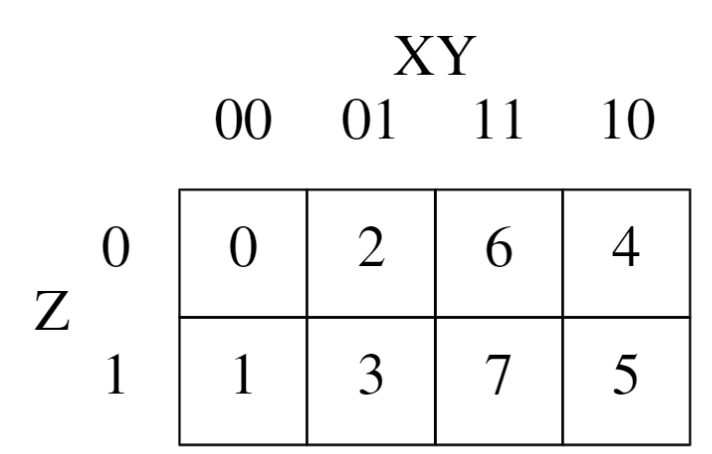
\includegraphics[width = 150px]{images/karnaugh.png}
\end{center}
where the numbers represent the minterms of the function. This can be expanded to more variables, by dividing the number of variables by two.\\
The order of the bits on each side of the rectangle is the gray code for that amount of bits. That is, after dividing the number of bits by two, to get the number of bits on each side of the rectangle, we will assign the bits, and organize the binary values in gray code order. This allows for only one bit to change between two adjacent cells. This will allow for simlification using the $(A\land X\lor(A\land X')) = A$.\\
\textit{Note: to generate n-bit gray code the following steps can be followed:
    \begin{itemize}
        \item Write out $0$ n times. This will be your first bit.
        \item Change the least significant but to 1. You will now have $000...01$
        \item Reflect this pair of bits, but change the 2-bit to $1$. You will generate a
              pair $00...11$,$00...10$.
        \item Reflect all the bits you have, and change the next most significant bit from
              $0$ to $1$, until you have all $2^n$ combinations.\\ Example for n=4, with each
              horizontal line being a reflection:
              \begin{table}
                  \centering
                  \begin{tabular}{c}
                      0000 \\
                      0001 \\
                      \hline
                      0011 \\
                      0010 \\
                      \hline
                      0110 \\
                      0111 \\
                      0101 \\
                      0100 \\
                      \hline
                      1100 \\
                      1101 \\
                      \vdots
                  \end{tabular}
              \end{table}
    \end{itemize}
}
So, the function $F(X,Y,Z) = \sum_{X,Y,Z}(3,6,7)$ would be represented as
\begin{center}
    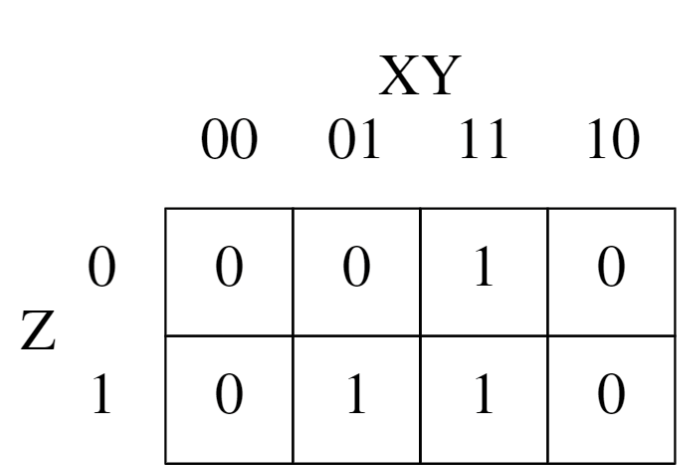
\includegraphics[width = 150px]{images/Karnaugh_use.png}
\end{center}
Let us assume we have a completed Karnaugh map. We will now observe adjacent terms, if there are two adjacent ones, be it vertical (6,7), horizontal (3,7), or across borders (4,0), they can be combined using the combining theorems.\\
\begin{center}
    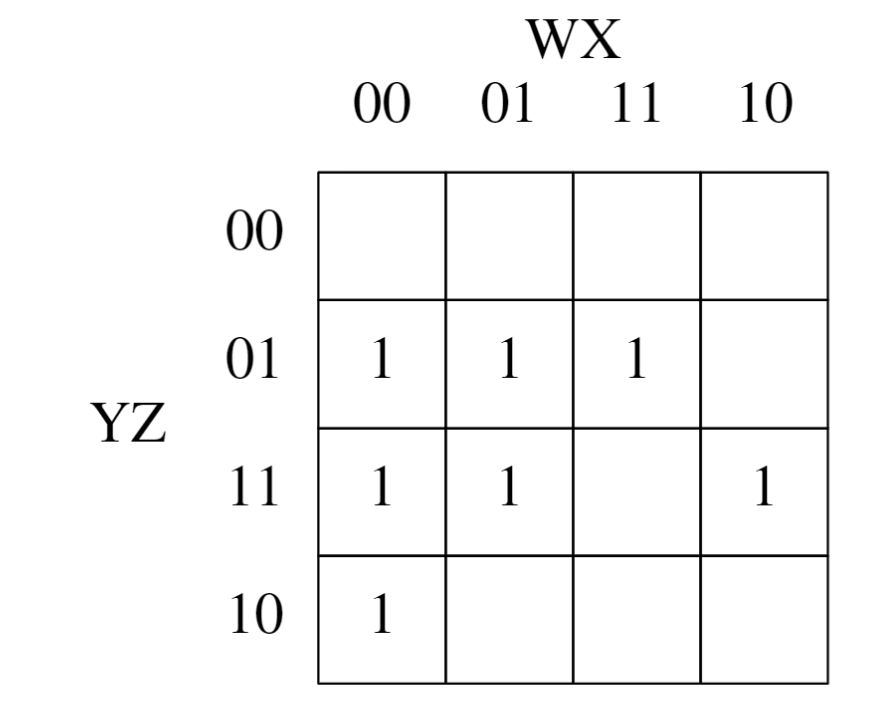
\includegraphics[width = 150px]{images/karnaugh4example.png}
\end{center}
So, in the above Karnaugh map, any of the following can be combined:
\begin{center}
    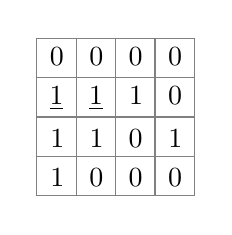
\begin{tikzpicture}
        \draw[step=0.5cm,color=gray] (-1,-1) grid (1,1);
        \matrix[matrix of nodes,nodes={inner sep=0pt,text width=.5cm,align=center,minimum height=.5cm}]{
            0             & 0             & 0 & 0 \\
            \underline{1} & \underline{1} & 1 & 0 \\
            1             & 1             & 0 & 1 \\
            1             & 0             & 0 & 0 \\
        };
    \end{tikzpicture}
    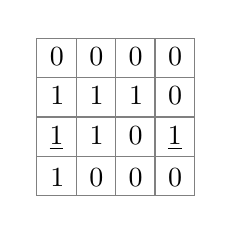
\begin{tikzpicture}
        \draw[step=0.5cm,color=gray] (-1,-1) grid (1,1);
        \matrix[matrix of nodes,nodes={inner sep=0pt,text width=.5cm,align=center,minimum height=.5cm}]{
            0             & 0 & 0 & 0             \\
            1             & 1 & 1 & 0             \\
            \underline{1} & 1 & 0 & \underline{1} \\
            1             & 0 & 0 & 0             \\
        };
    \end{tikzpicture}
    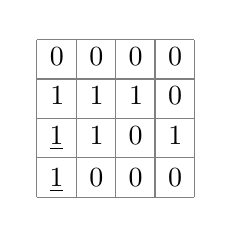
\begin{tikzpicture}
        \draw[step=0.5cm,color=gray] (-1,-1) grid (1,1);
        \matrix[matrix of nodes,nodes={inner sep=0pt,text width=.5cm,align=center,minimum height=.5cm}]{
            0             & 0 & 0 & 0 \\
            1             & 1 & 1 & 0 \\
            \underline{1} & 1 & 0 & 1 \\
            \underline{1} & 0 & 0 & 0 \\
        };
    \end{tikzpicture}
\end{center}
Additionally, if you combine two ones, you can then combine an adjacent pair:
\begin{center}
    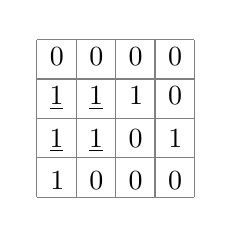
\begin{tikzpicture}
        \draw[step=0.5cm,color=gray] (-1,-1) grid (1,1);
        \matrix[matrix of nodes,nodes={inner sep=0pt,text width=.5cm,align=center,minimum height=.5cm}]{
            0             & 0             & 0 & 0 \\
            \underline{1} & \underline{1} & 1 & 0 \\
            \underline{1} & \underline{1} & 0 & 1 \\
            1             & 0             & 0 & 0 \\
        };
    \end{tikzpicture}
\end{center}
So, all four of the above ones can be combined into a single term.\\
\textit{Note: each combination will have $2^n$ terms.}\\
The goal is to combine as many terms as possible.\\
This leads to the following rules:
\begin{itemize}
    \item If combinations cover only areas of the map where the variable is 0, the
          variable is complemented in the product term.
    \item If combinations cover only areas of the map where the variable is 1, the
          variable is uncomplemented in the product term.
    \item If combinations cover all areas of the map where a variable is either 0 or 1,
          the term does not appear
\end{itemize}
We want as few combinations as possible, and these combinations to be as large as possible.\\
The remaining products are then added together.\\
The above map will have the following combinations:\\
\begin{center}
    \begin{table}
        \begin{tabular}{c c c c}

            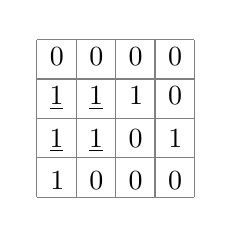
\begin{tikzpicture}
                \draw[step=0.5cm,color=gray] (-1,-1) grid (1,1);
                \matrix[matrix of nodes,nodes={inner sep=0pt,text width=.5cm,align=center,minimum height=.5cm}]{
                    0             & 0             & 0 & 0 \\
                    \underline{1} & \underline{1} & 1 & 0 \\
                    \underline{1} & \underline{1} & 0 & 1 \\
                    1             & 0             & 0 & 0 \\
                };
            \end{tikzpicture} &
            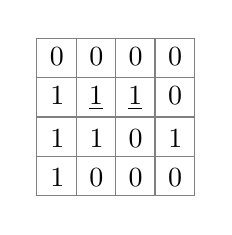
\begin{tikzpicture}
                \draw[step=0.5cm,color=gray] (-1,-1) grid (1,1);
                \matrix[matrix of nodes,nodes={inner sep=0pt,text width=.5cm,align=center,minimum height=.5cm}]{
                    0 & 0             & 0             & 0 \\
                    1 & \underline{1} & \underline{1} & 0 \\
                    1 & 1             & 0             & 1 \\
                    1 & 0             & 0             & 0 \\
                };
            \end{tikzpicture} &
            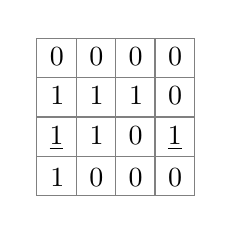
\begin{tikzpicture}
                \draw[step=0.5cm,color=gray] (-1,-1) grid (1,1);
                \matrix[matrix of nodes,nodes={inner sep=0pt,text width=.5cm,align=center,minimum height=.5cm}]{
                    0             & 0 & 0 & 0             \\
                    1             & 1 & 1 & 0             \\
                    \underline{1} & 1 & 0 & \underline{1} \\
                    1             & 0 & 0 & 0             \\
                };
            \end{tikzpicture} &
            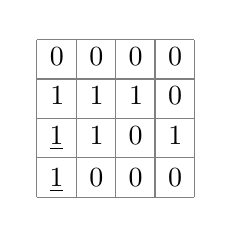
\begin{tikzpicture}
                \draw[step=0.5cm,color=gray] (-1,-1) grid (1,1);
                \matrix[matrix of nodes,nodes={inner sep=0pt,text width=.5cm,align=center,minimum height=.5cm}]{
                    0             & 0 & 0 & 0 \\
                    1             & 1 & 1 & 0 \\
                    \underline{1} & 1 & 0 & 1 \\
                    \underline{1} & 0 & 0 & 0 \\
                };
            \end{tikzpicture}                                                                     \\
            $W'\land Z$                                                & $X\land Y' \land Z$ & $X'\land Y\land Z$ & $W'\land X'\land Y$ \\
            \hline
            \begin{tabular}{c|c}
                W & 00 \\
                X & 01 \\
                Y & 10 \\
                Z & 11
            \end{tabular}                                       &
            \begin{tabular}{c|c}
                W & 01 \\
                X & 11 \\
                Y & 0  \\
                Z & 1
            \end{tabular}                                       &
            \begin{tabular}{c|c}
                W & 10 \\
                X & 00 \\
                Y & 1  \\
                Z & 1
            \end{tabular}                                       &
            \begin{tabular}{c|c}
                W & 0  \\
                X & 0  \\
                Y & 11 \\
                Z & 10
            \end{tabular}
        \end{tabular}
    \end{table}
\end{center}
Each of these resulting combinations will result in a single product.
Based on the aforementioned rules, it will be defined as: \\~\\$(W' \land Z) \lor (X\land Y' \land Z) \lor (X'\land Y\land Z) \lor (W'\land X'\land Y)$\\~\\
    A logic function implies another if for every function in which the first function is 1, the second function is 1 as well. This is called an implicant.\\
    A prime implicant is one such that if any variable is dropped from its product term would stop it from being an implicant. That is, if the combination was once again combined, it no longer only combines 1's.
    This leads to the prime implicant theorem, which tells us that a minimal sum is a sum of prime implicants. So, to find a minimal sum we only need to consider it's prime implicants.\\
    It is possible for a function to have more prime implicants than the number of necessary terms in the minimal sum. So, we will add another few definitions:\\
    \begin{itemize}
        \item A distinguished minterm of a logic function is a minterm covered by only one
              prime implicant.
        \item An essential prime implicant is a prime implicant that covers one or more
              distinguished minterms.
    \end{itemize}
    These two definitions allow us to find the minimal sum through the following steps:
    \begin{enumerate}
        \item Find all the prime implicants
        \item Identify the distinguished minters and essential prime implicants.
        \item Include all the essential prime implicants.
    \end{enumerate}
    But, this will not assure covering all the ones. So, we make an additional rule:\\
    If P and Q are prime implicants and the number of literals in P is not greater than the number in Q and P covers all the remaining minterms in Q, remove Q.\\
    Some of the remaining may be necessary to select. These are secondary prime implicants.\\
    So we are going to create a prime implicant table:\\
    \begin{itemize}
        \item A row for every prime implicant
        \item A column for every minterm
        \item A mark if the corresponding implicant covers the corresponding minterm
    \end{itemize}
    So, for\\
    \begin{center}
        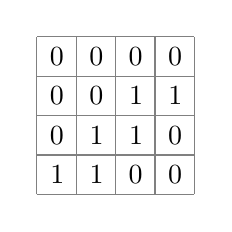
\begin{tikzpicture}
            \draw[step=0.5cm,color=gray] (-1,-1) grid (1,1);
            \matrix[matrix of nodes,nodes={inner sep=0pt,text width=.5cm,align=center,minimum height=.5cm}]{
                0 & 0 & 0 & 0 \\
                0 & 0 & 1 & 1 \\
                0 & 1 & 1 & 0 \\
                1 & 1 & 0 & 0 \\
            };
        \end{tikzpicture}
    \end{center}
    the table would be:
    \begin{center}
        \begin{table}
            \centering
            \begin{tabular}{c|c c c c c c}
                     & 0010 & 0110 & 0111 & 1001 & 1101 & 1111 \\
                \hline
                1-01 &      &      &      & x    & x    &      \\
                -111 &      &      & x    &      &      & x    \\
                0-10 & x    & x    &      &      &      &      \\
                011- &      & x    & x    &      &      &      \\
                11-1 &      &      &      &      & x    & x    \\
            \end{tabular}
        \end{table}
    \end{center}
    If there is a column with only one mark, it's implicant is selected. All the marks it covers are selected, and these columns and rows are removed.\\
    \begin{center}
        \begin{table}
            \centering
            \begin{tabular}{c|c c c c c c}
                                 & \underline{0010} & \underline{0110} & 0111 & \underline{1001} & \underline{1101} & 1111 \\
                \hline
                \underline{1-01} &                  &                  &      & \underline{x}    & \underline{x}    &      \\
                -111             &                  &                  & x    &                  &                  & x    \\
                \underline{0-10} & \underline{x }   & \underline{x}    &      &                  &                  &      \\
                011-             &                  & x                & x    &                  &                  &      \\
                11-1             &                  &                  &      &                  & x                & x    \\
            \end{tabular}
        \end{table}
    \end{center}
    \pagebreak
    The table above is reduced to:\\
    \begin{center}
        \begin{table}
            \centering
            \begin{tabular}{c| c c}
                     & 0111 & 1111 \\
                \hline
                -111 & x    & x    \\
                011- & x    &      \\
                11-1 &      & x    \\
            \end{tabular}
        \end{table}
    \end{center}
    Since -111 covers both the others, they can be removed, and we keep -111.\\
    This process can be conducted several times, until it is as reduced as possible. However, the Karnaugh map is not powerful enough to always get the minimal form. That will require another representation. However, for several cases, it will drastically reduce the number of terms in the prime implicant table.\\
    This process can instead be conducted for zeros, or considering $F'$, and using deMorgan's on the result.
    \subsection{Quine-McCluskey Method}
    This method is also based on the $A\land X \lor A\land X' = A$.\\ We start by
    listing out all the minterms, for example, for $F(W,X,Y,Z) = \sum
(2,6,7,9,13,15)$:\\
    \begin{table}
        \centering
        \begin{tabular}{c c}
            2  & 0010 \\
            \hline
            6  & 0110 \\
            9  & 1001 \\
            \hline
            7  & 0111 \\
            13 & 1101 \\
            \hline
            15 & 1111
        \end{tabular}
    \end{table}
    Note how the terms are divided by the number of ones in the binary of the minterm.\\
    We will then combine each pair of consecutive sections, all terms with all terms:\\
    \begin{table}
        \centering
        \begin{tabular}{c c}
            2,6   & 0-10 \\
            \hline
            6,7   & 011- \\
            9,13  & 1-01 \\
            \hline
            7,15  & -111 \\
            13,15 & 11-1 \\
        \end{tabular}
    \end{table}
    Two minterms are combined if there is only one bit of difference between the two. The process would be continued if this could be done again, that is, if there were terms in consecutive sections with only one bit difference between two items in two consecutive sections. We will mark every expression that has been combined, and thus appears in a lower table. If there is one that is not selected, and thus unmarked, it will be a part of the final prime implicant table.\\
    \begin{mdframed}
        \textbf{Incompletely Specified Functions}\\
        These are functions in which we know what the output should be for certain inputs but don't care what it is for other inputs. To deal with them, the prime implicants can optionally cover them, and occasionally make more efficient expressions.\\
        So, the following map:\\
        \begin{center}
            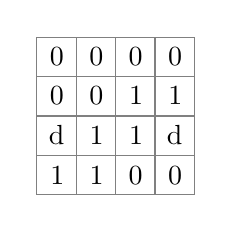
\begin{tikzpicture}
                \draw[step=0.5cm,color=gray] (-1,-1) grid (1,1);
                \matrix[matrix of nodes,nodes={inner sep=0pt,text width=.5cm,align=center,minimum height=.5cm}]{
                    0 & 0 & 0 & 0 \\
                    0 & 0 & 1 & 1 \\
                    d & 1 & 1 & d \\
                    1 & 1 & 0 & 0 \\
                };
            \end{tikzpicture}
        \end{center}
        can have any values at the d, that is, it can be 0 or 1.\\ So, if we were to select them both as one, the final expression would only have two terms instead of three.
        \begin{center}
            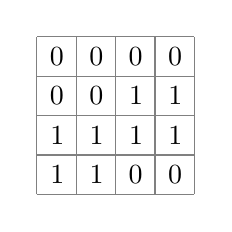
\begin{tikzpicture}
                \draw[step=0.5cm,color=gray] (-1,-1) grid (1,1);
                \matrix[matrix of nodes,nodes={inner sep=0pt,text width=.5cm,align=center,minimum height=.5cm}]{
                    0 & 0 & 0 & 0 \\
                    0 & 0 & 1 & 1 \\
                    1 & 1 & 1 & 1 \\
                    1 & 1 & 0 & 0 \\
                };
            \end{tikzpicture} $\rightarrow$
            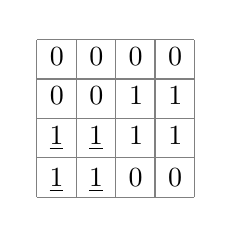
\begin{tikzpicture}
                \draw[step=0.5cm,color=gray] (-1,-1) grid (1,1);
                \matrix[matrix of nodes,nodes={inner sep=0pt,text width=.5cm,align=center,minimum height=.5cm}]{
                    0             & 0             & 0 & 0 \\
                    0             & 0             & 1 & 1 \\
                    \underline{1} & \underline{1} & 1 & 1 \\
                    \underline{1} & \underline{1} & 0 & 0 \\
                };
            \end{tikzpicture}
            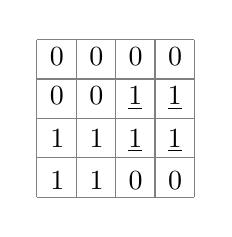
\begin{tikzpicture}
                \draw[step=0.5cm,color=gray] (-1,-1) grid (1,1);
                \matrix[matrix of nodes,nodes={inner sep=0pt,text width=.5cm,align=center,minimum height=.5cm}]{
                    0 & 0 & 0             & 0             \\
                    0 & 0 & \underline{1} & \underline{1} \\
                    1 & 1 & \underline{1} & \underline{1} \\
                    1 & 1 & 0             & 0             \\
                };
            \end{tikzpicture}
        \end{center}
    \end{mdframed}
    The table that is drawn with incompletely specified functions represents terms we don't care about as dashes.\\
    The prime implicant table will also not include the "don't-care" terms. We will conduct the same process as what was done for earlier prime implicant tables.\\
    \section{Timing Hazards}
    The output of a gate is not instant, and the delay could possibly cause errors
    in the output if the delay is severe enough.\\ Suppose there is a change in an
    input to a gate, through which there is an expected change in the output, which
    will be delayed, and can thus cause problems.\\ This erroneous performance is
    called a glitch, and the probability of it happening, is called the hazard.\\
    \subsection{Static Hazards}
    \begin{mdframed}
        \textbf{Static Hazards}\\
        The static-1 hazard is the possibility that the circuit will have a momentary 0 pulse when it is supposed to be stable at 1.\\
        It is a pair of input combinations that differ in only one input variable and they both give a 1 output, causing a momentary 0.\\
        The reason for these conditions is that it is possible for only one input to change at a time.\\
        The same can happen for 0, which would be called a static-0 hazard.\\
        Only one input changes in a static hazard.
    \end{mdframed}
    K-maps can be used to locate static hazards. We look for prime implicants that are adjacent, and the change between them is not covered by the circuit.\\
    \begin{center}
        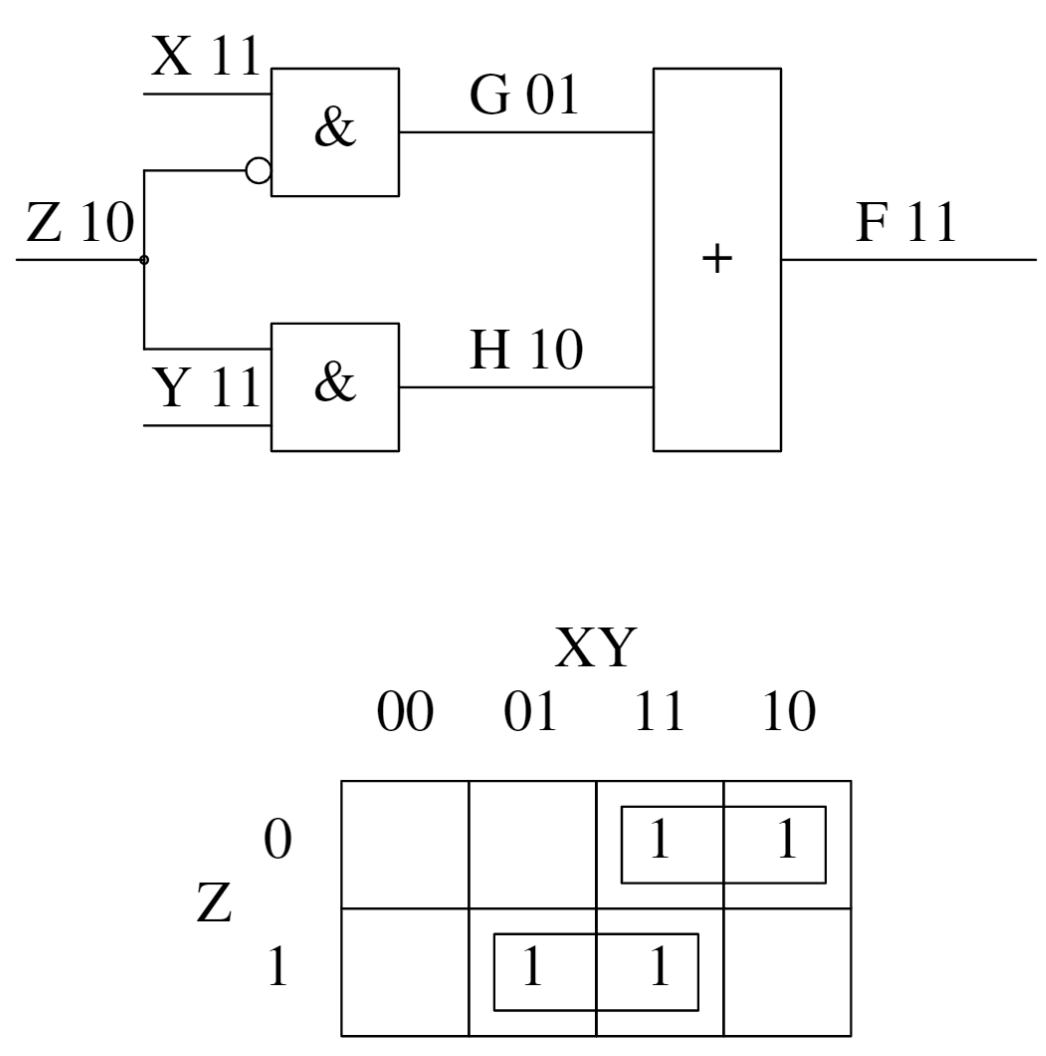
\includegraphics[width = 150px]{images/kmaphazard.png}
    \end{center}
    The upper prime implicant and the lower prime implicant, which are each covered by AND gates, have the $11$ column as an adjacency. This can cause timing hazards to occur. To fix them, one would be to add the hazard causing adjacency as an additional AND gate to the circuit.\\
    \begin{center}
        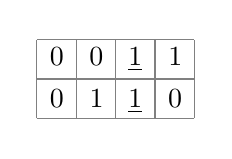
\begin{tikzpicture}
            \draw[step=0.5cm,color=gray] (-1,-0.5) grid (1,0.5);
            \matrix[matrix of nodes,nodes={inner sep=0pt,text width=.5cm,align=center,minimum height=.5cm}]{
                0 & 0 & \underline{1} & 1 \\
                0 & 1 & \underline{1} & 0 \\
            };
        \end{tikzpicture}
    \end{center}
    If were to not use a K-map, we would need to compare all pairs of prime implicants and find terms that differ in the value of a single input.\\
    If there are no adjacent K-map terms, or all the items that need to be covered, are already covered, no timing hazard will occur.
    \subsection{Dynamic Hazards}
    \begin{mdframed}
        \textbf{Dynamic Hazards}\\
        They are the possibility of an output changing multiple times based on a single input change.\\
        This needs to be a multilevel circuit.\\
        The dynamic hazard occurs because there was a static hazard in one of its inputs. This causes its value to change temporarily before its final output.\\
        So, in essence, if there is a difference in the beginning output and the end output, and a glitch in the process, it would be a dynamic hazard.
    \end{mdframed}
    To analyze the hazards on a multilevel circuit, we analyze each of the inputs, and mark where there are changes:
    \begin{table}
        \centering
        \begin{tabular}{|c|c c|}
            W & 0 & 0 \\
            X & 0 & 1 \\
            Y & 0 & 0 \\
            Z & 1 & 1 \\
        \end{tabular} $\rightarrow$
        \begin{tabular}{|c|c c c|}
            W & 0 & 0 & 0 \\
            X & 0 & x & 1 \\
            Y & 0 & 0 & 0 \\
            Z & 1 & 1 & 1 \\
        \end{tabular}
    \end{table}
    The analysis is done with the second set of inputs. All the inputs to each gate are analyzed. If there is an x in between a $0$ and a $1$ at any output, there is no hazard. However, if at some output there is an x in between $1$ and $1$, or between $0$ and $0$, there would be a static hazard at that output. Any gate that has this as an input, will then have a dynamic hazard at its output.
    \section{Digital Circuits}
    \defn{Static behavior}{situations where inputs are not changing.}\\
    \defn{Dynamic Behavior}{situations with changing inputs.}\\
    \defn{Fan-in}{The maximum number of inputs a gate can have in some predefined logic family, is defined as the fan-in of the logic family.}\\
    So, for the CMOS family, the fan-in would ideally be $\infty$, but, because the resistance of the transistors starts mounting, there is a limit.\\
In the CMOS family, the fan-in for a NAND gate is 6, and for a NOR it is 4.\\
If we wanted more inputs, we would need to connect multiple gates.\\
\subsection{CMOS Static Electrical Behavior}
Before, we had:
\begin{table}
    \centering
    \begin{tabular}{c|c}
        $V_{in}$ & $V_{out}$ \\
        \hline
        0V       & 5V        \\
        5V       & 0V
    \end{tabular}
\end{table}
But the graph is actually slanted. This introduces new parameters that the manufacturer provides.\\
\begin{itemize}
    \item \defn{$V_{OHmin}$}{The minimum output at HIGH.}
    \item \defn{$V_{IHmin}$}{The minimum input that will be recognized HIGH.}
    \item \defn{$V_{OLmax}$}{The maximum output at LOW.}
    \item \defn{$V_{ILmax}$}{The maximum input to be recognized as LOW.}
\end{itemize}
\defn{DC noise margin}{amount of noise to corrupt the worst case output to not be recognized properly.\\
    \quad For LOW:
    \begin{equation*}
        V_{ILMax} - V_{OLmax}
    \end{equation*}
    \quad For HIGH:
    \begin{equation*}
        V_{OHmin} - V_{IHmin}
    \end{equation*}
}
CMOS gates also have something known as leakage current, which is caused by the input consuming current when it would ideally not be doing so.\\
\begin{itemize}
    \item $I_{IL}$: the maximum current flowing when it is LOW.
    \item $I_{IH}$: the maximum current flowing when it is HIGH.
\end{itemize}
If a circuit is not purely CMOS, or if there are high resistances in other parts of the circuit, there would be a need to model the resistance of the output.
This causes the outputs to be slightly lower or higher than what it should be at that state.\\
\begin{itemize}
    \item \defn{$I_{OLmax}$}{Maximum current an output can sink if while maintaining the voltage below $V_{OLmax}$.}
    \item \defn{$I_{OHmin}$}{Minimum current an output needs to maintain the voltage above $V_{OHmin}$.}
\end{itemize}
\defn{Fan-out}{Number of inputs the gate can drive without exceeding worst case specs.}\\
It is calculated as: $\min((V_{OLMax}/V_{IL}), (V_{OHmax}/V_{IH}))$.\\
If the fan-out is surpassed, there are several effects, such as longer delays, noise, etc. that will affect the functionality of the circuit.
\subsection{CMOS Dynamic Electrical Behavior}
This determines the speed and power consumption of the circuit.\\
\defn{Transition Time}{amount of time taken to change of one voltage level to another.}\\
Till now, we had modeled circuits with right angles, but transitions are actually slanted, and, in fact, the slope change is also continuous.\\
\begin{center}
    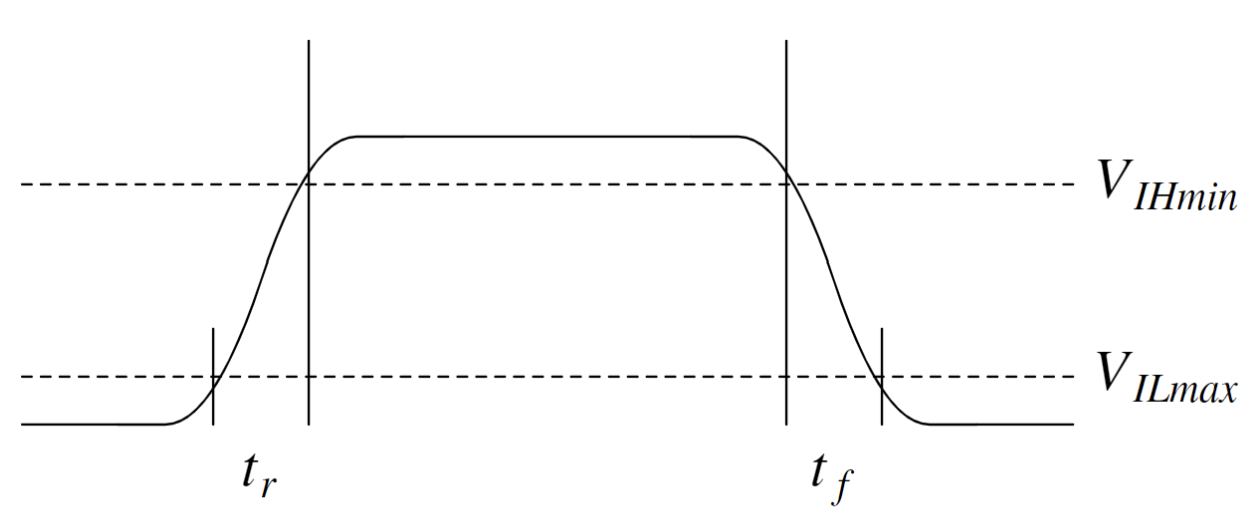
\includegraphics[width = 200px]{images/tdelaygraph.png}
\end{center}
These times depend on the resistances of the transistors, the capacitances in the system, among others.\\
The following equation will allow us to calculate the delay from low to high.
\begin{align*}
    V_{OUT} = V_{CC}e^{-t/(R_n C_L)}
\end{align*}
The same principle can be used to calculate in the other direction.\\
\defn{Propagation Delay}{amount of time it takes for a change in the input signal to cause a change in the output signal.}\\
\defn{$t_{pHL}$}{time between an input change and the corresponding output changes from HIGH to LOW.}\\
\defn{$t_{pLH}$}{time between an input change and the corresponding output changes from LOW to HIGH.}\\
\begin{center}
    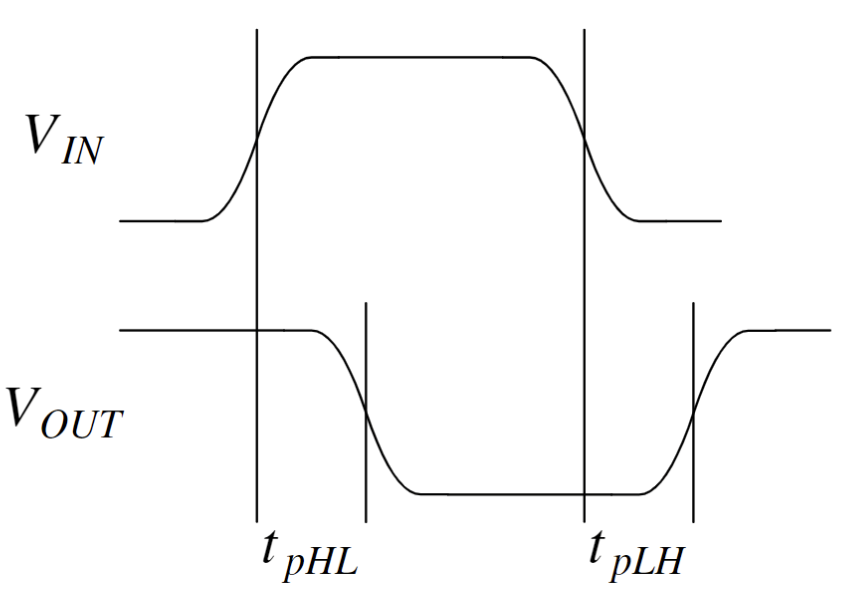
\includegraphics[width = 200px]{images/propdelaygraph.png}
\end{center}
\begin{mdframed}
    \textbf{Slight Side topics}\\
    Power consumption:  If the inputs are not changing, it is called static power consumtpion.\\
    CMOS circuits have very low power consumption.\\
    Decoupling capacitors allow for reduction of current spikes.\\
    Wires or connections may have an inductance, allowing for voltage drops.\\
\end{mdframed}
\subsection{Tri-State Outputs}
    This allows for the creation of a gate that allows for the gate to behave as if it is not in the circuit. That is, it behaves as an open circuit.\\
    This will allow for multiple gates driving a bus, with all but one disconnected, allowing this one to write the output of the bus.\\
    This is essentially adding an enabled/disabled state:
    \begin{center}
        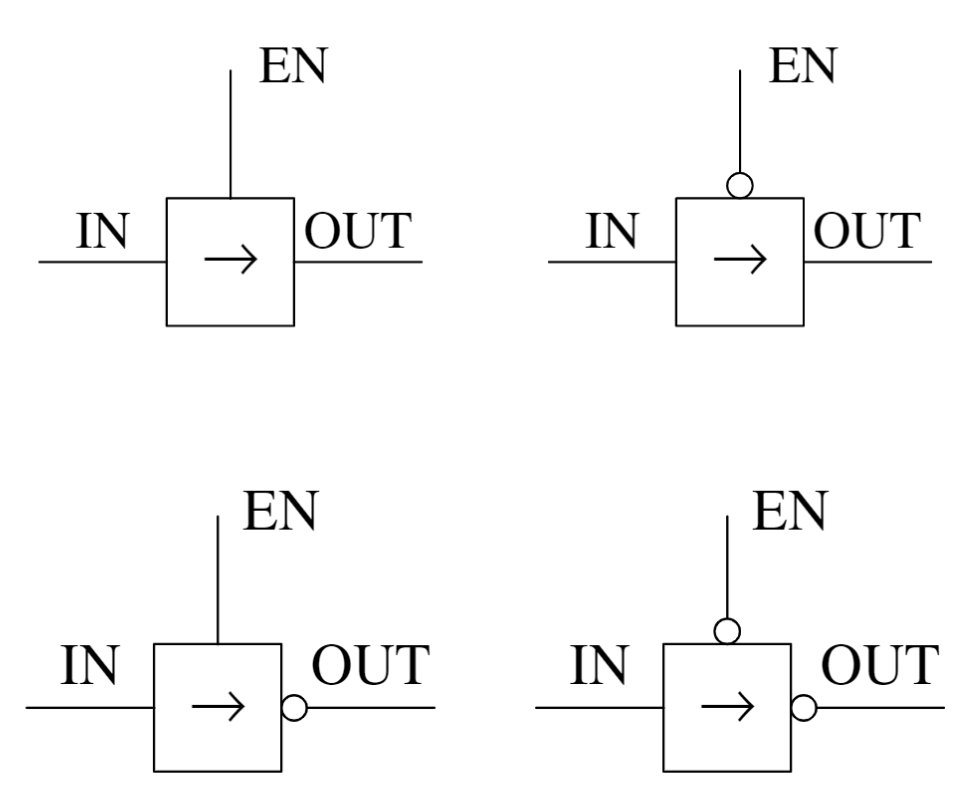
\includegraphics[width = 200px]{images/enable_gates.png}
    \end{center}
   The first of the above gates is created through the following circuit:
    \begin{center}
        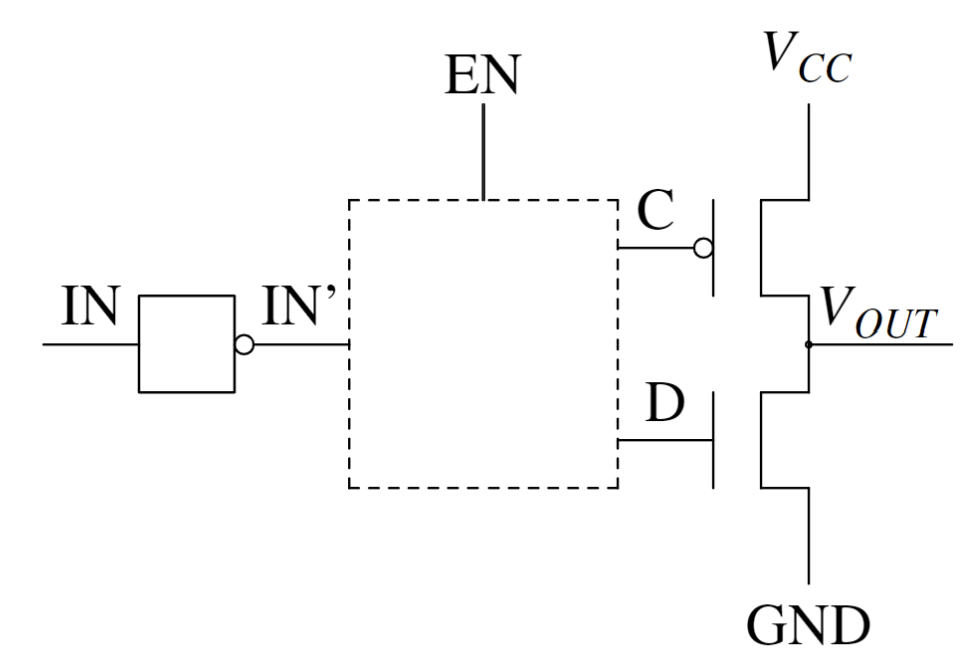
\includegraphics[width = 200px]{images/enable_circuit.png}
    \end{center}
    If enable is 0, the resistance of the circuit goes to a very high value, making it not exist to the rest of the circuit.\\
    The "blackbox" in the circuit is the $(C\land D')\lor(C\land D)'$.\\
    So, in the situation above, one could enable or disable these at will. When this is disabled, it will act as a third state, that of "nonexistence".\\~\\
    Tri-State outputs are designed so that the output enable delay is longer than the disable delay. This will allow us to avoid there being two or more inputs into a bus to be enabled at the same time.\\
    However, this may not always be possible.\\
    So we create a solution that makes sure there is a disable for everything between any two enables. This will allow us to make sure there is never a conflict due to this.\\
    \defn{Bus Transceiver}{device used to connect two buses, allowing them to write to each other.}\\
    The following is an example of transceivers being used:
    \begin{center}
        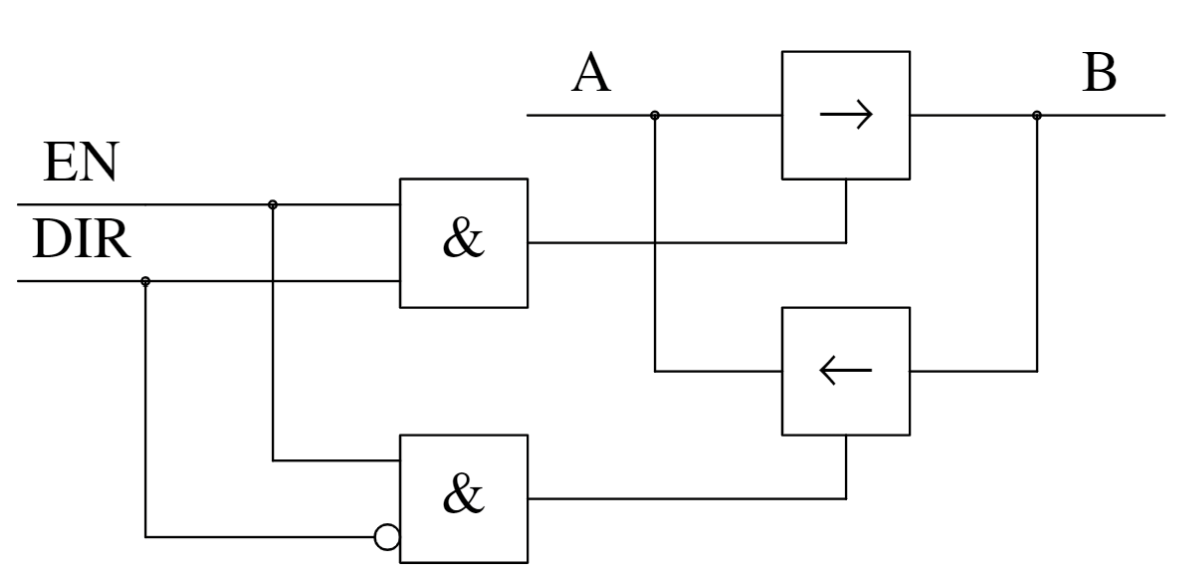
\includegraphics[width = 200px]{images/transcieveruse.png}
    \end{center}
    \begin{table}
        \centering
        \begin{tabular}{c|c|c}
            EN-DIR & Mode & Operation\\
            \hline
            0-x & disconnect & disconnect\\
            1-0 & 0 & A writes to B\\
            1-1 & 1 & B writes to A
            
        \end{tabular}
    \end{table}
    There is also a leakage current here, that must be taken into account.
\section{Complex CMOS Gates}
If we were to analyze the following circuit:
\begin{center}
    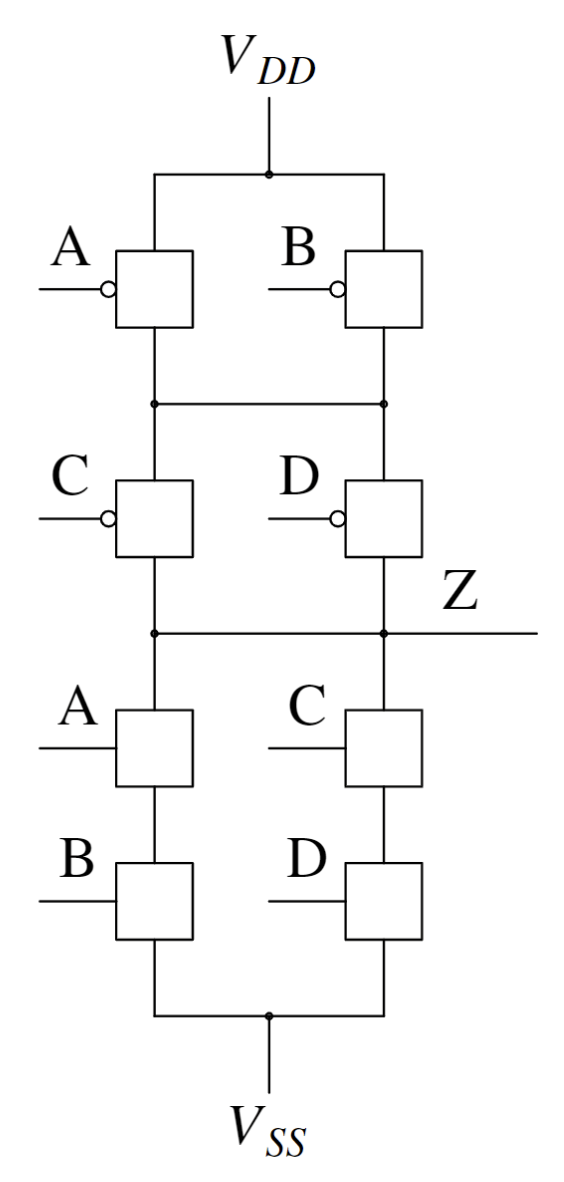
\includegraphics[width = 75px]{images/complexcmos.png}
\end{center}
We must analyze what situations will lead to a connection between $Z$ and $V_{DD}$ or $V_{SS}$. Series basically represents AND ($\land$), while parallel basically represents OR ($\lor$).\\
So the above function is $(A'\lor B')\land(C'\lor D')$, as those are the combinations that will lead to Z to be connected to HIGH, or $V_{DD}$.
Transmission gates are essentially switches controlled by enables.\\
\begin{center}
    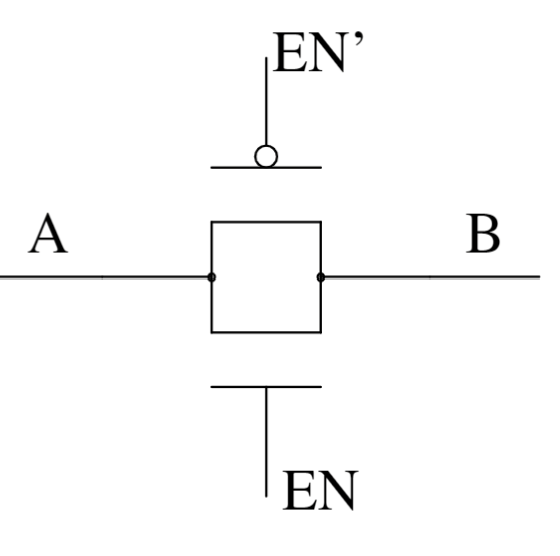
\includegraphics[width = 100px]{images/transmission_gate.png}
\end{center}
It is a PMOS connected with and NMOS that are connected through complementing control signals. When EN is LOW, both of them are off, and thus the circuit is disconnected. When EN is HIGH, both of them are on, and thus the circuit is connected.\\
The reason we have two gates, instead of just one to connect A and B, is because NMOS transistors are not good at transmitting HIGH voltages, and PMOS are not good at transmitting LOW voltages. However, together, both HIGH and LOW can be transmitted.\\
\end{document}